\chapter{Analisi}
\label{Cha:analisi}
\thispagestyle{empty}

Il capitolo seguente sarà incentrato sulla presentazione dei prodotti, seguita da una descrizione generale degli algoritmi utilizzati per effettuare le rispettive analisi.

\section{Prodotti}
Per gli esperimenti sono stati usati tre tipi di battistrada diversi. I primi due (figura \ref{fig:batt_1a} e figura \ref{fig:batt_1b})sono molto simili ma differenziano per complessità e numero di blocchi (\textit{blob}), mentre il terzo (figura \ref{fig:batt_2}) è molto differente perchè presenta delle concavità irregolari e delle parti consumate.\\
Da questo momento in poi, per facilitarne la comprensione, ogni battistrada avrà un suo nome specifico.\\

\begin{figure}[H]
	\centering
	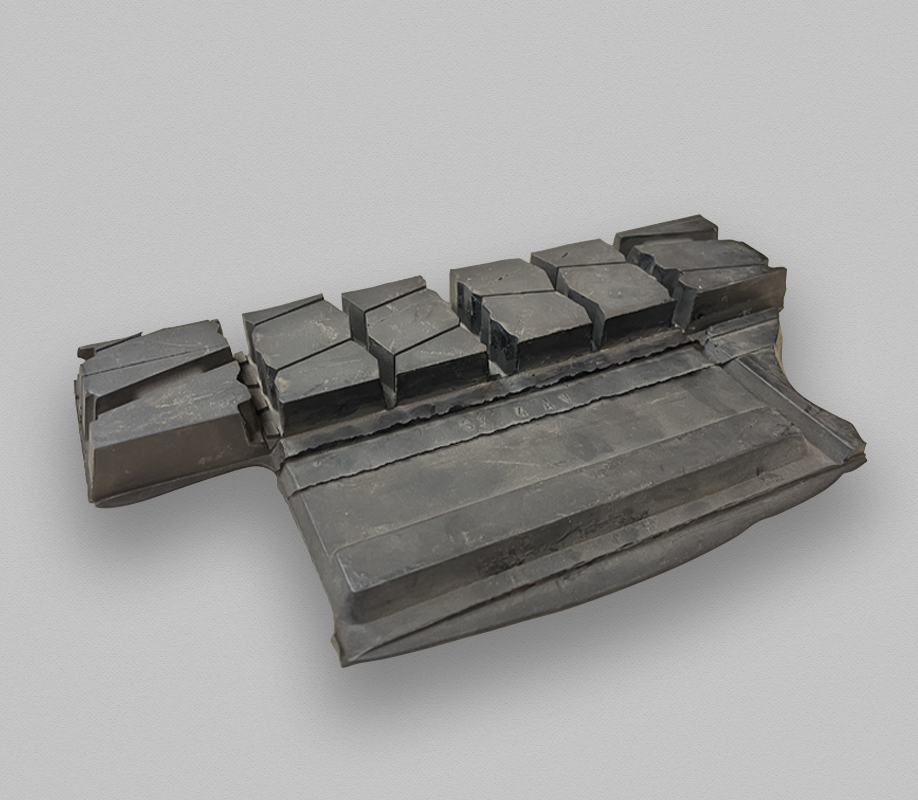
\includegraphics[height=0.41\columnwidth]{./pictures/batt_1a_1.png}
	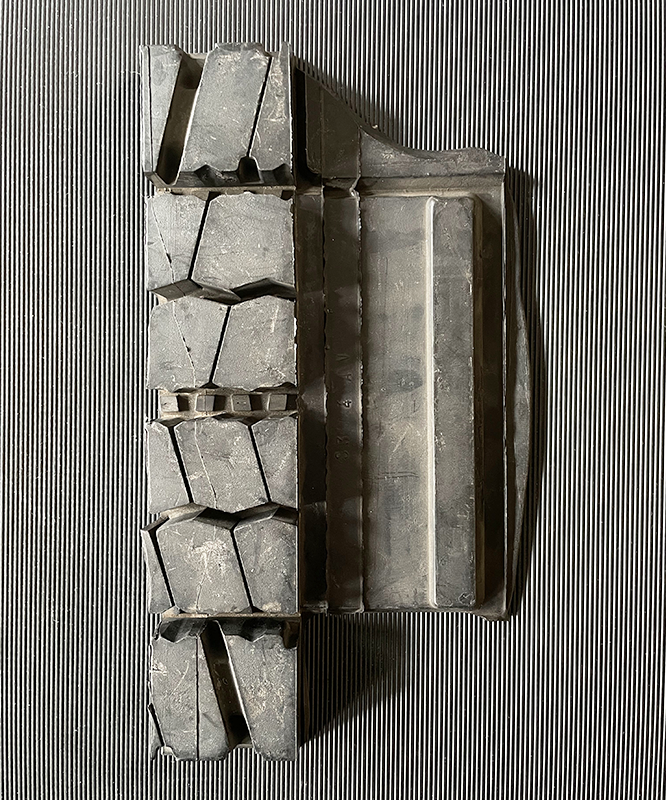
\includegraphics[height=0.41\columnwidth]{./pictures/batt_1a_2.png}
	\caption{Battistrada di tipo \textit{1A}}\label{fig:batt_1a}
\end{figure}

\begin{figure}[H]
	\centering
	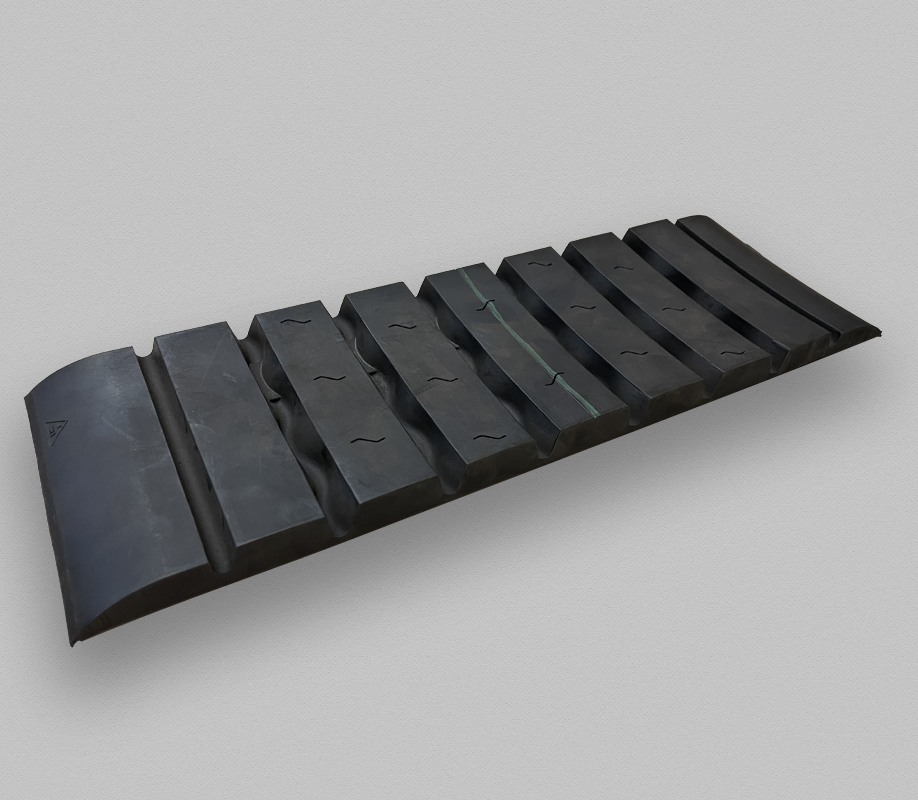
\includegraphics[height=0.41\columnwidth]{./pictures/batt_1b_1.png}
	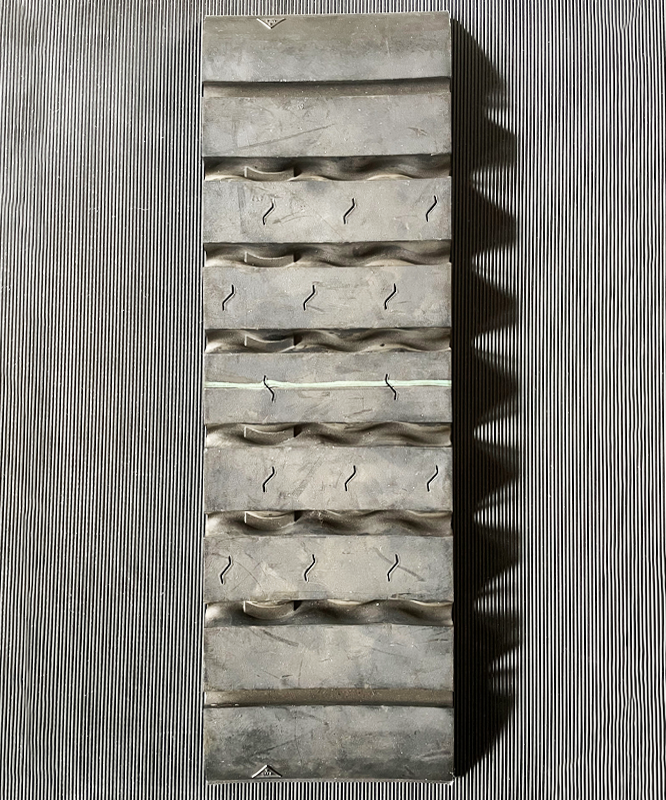
\includegraphics[height=0.41\columnwidth]{./pictures/batt_1b_2.png}
	\caption{Battistrada di tipo \textit{1B}}\label{fig:batt_1b}
\end{figure}

\begin{figure}[H]
	\centering
	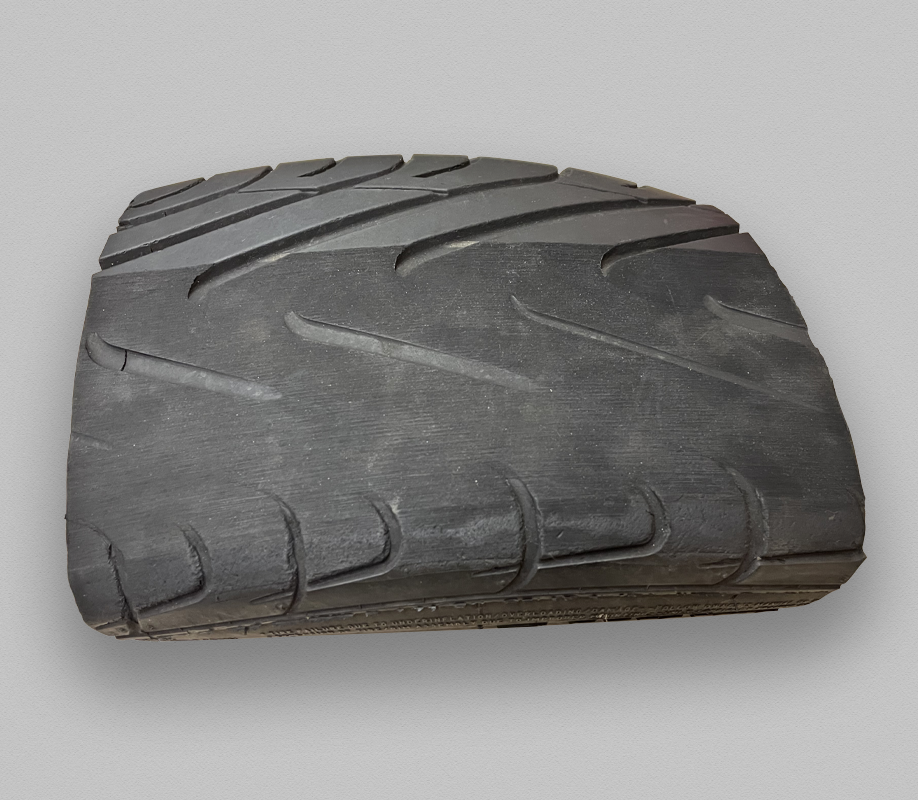
\includegraphics[height=0.41\columnwidth]{./pictures/batt_2_1.png}
	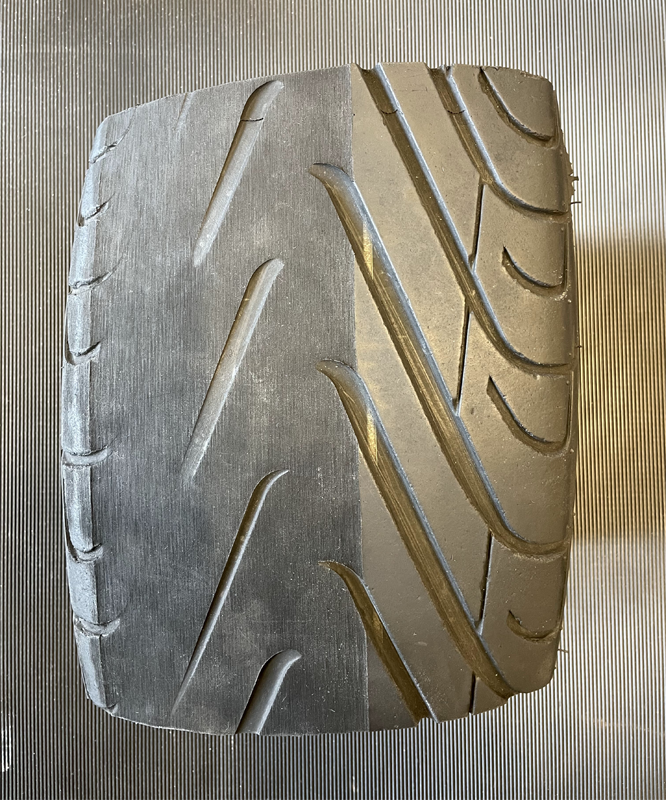
\includegraphics[height=0.41\columnwidth]{./pictures/batt_2_2.png}
	\caption{Battistrada di tipo \textit{2}}\label{fig:batt_2}
\end{figure}

\newpage

\section{Librerie di supporto}
Il programma è stato creato in \textit{C++} e in \textit{C\#}, utilizzando \textit{Visual Studio} come ambiente di sviluppo.\\
\newline
Le librerie utilizzate per realizzare il progetto sono:
\begin{itemize}
	\item \textit{Gocator Software Development Kit (GoSDK), versione 6.1.32.12}, è una libreria open source che può essere utilizzata per accedere e controllare a livello di codice i sensori del Gocator;
	\item \textit{OpenCV, versione 4.5.4}, è una libreria software multipiattaforma nell'ambito della visione artificiale in tempo reale;
	\item \textit{Point Cloud Library, versione 1.12.1}, è una libreria open source di algoritmi per le attività di elaborazione delle nuvole di punti e l'elaborazione della geometria 3D;
	\item \textit{GNU Scientific Library, versione 2.7}, è una libreria di software per calcoli numerici in matematica e scienze applicate;
	\item \textit{JSON for Modern C++, versione 3.10.5}, è una libreria per elaborare dati in formato \textit{JSON};
	\item \textit{Helix Toolkit, versione 2.20.2}, è una raccolta di componenti 3D per \textit{.NET};
	\item \textit{Json.NET - Newtonsoft, versione 13.0.1}, è un popolare framework JSON ad alte prestazioni per \textit{.NET};
	\item \textit{Ookii.Dialogs.Wpf, versione 5.0.1}, è una libreria per applicazioni \textit{WPF}.
\end{itemize}

\section{Algoritmi di analisi}

\subsection{Battistrada di tipo 1A/1B}
Dall'analisi di questo tipo di battistrada si è deciso di estrarre le seguenti features:
\begin{itemize}
	\item Distanza minima tra ogni \textit{MacroBlob} adiacente \textbf{(1A/1B)}.
	\item Area, perimetro e dimensione della \textit{bounding box} di ogni \textit{MacroBlob} \textbf{(1A/1B)}.
	\item Area, perimetro e dimensione della \textit{bounding box} di ogni \textit{Blob} \textbf{(1A)}.
	\item Per ogni \textit{MacroBlob}, la distanza minima tra ogni \textit{Blob} adiacente \textbf{(1A)}.
\end{itemize}

\noindent Successivamente, per fini statistici, si è calcolato il minimo, il massimo e la media dei valori trovati in elenco.\\
\newline
Prendendo come esempio il battistrada di tipo \textit{1A}, nella figura \ref{fig:batt_1a_analisi_mb} sono evidenziati i \textit{MacroBlob}, mentre nella figura \ref{fig:batt_1a_analisi_b} i \textit{Blob}.\\
Nel caso del battistrada di tipo \textit{1B} (figura \ref{fig:batt_1b_analisi_mb}), parliamo solo di \textit{MacroBlob} perchè non sono presenti blocchi interni.\\

\begin{figure}[H]
	\centering
	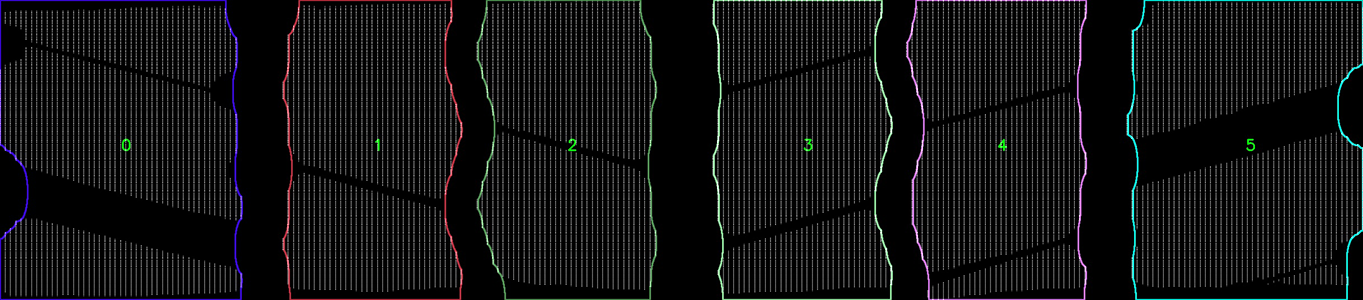
\includegraphics[width=0.9\columnwidth]{./pictures/batt_1a_analisi_mb.png}
	\caption{Contorni dei MacroBlob, in questo ne sono presenti 6.}\label{fig:batt_1a_analisi_mb}
\end{figure}

\begin{figure}[H]
	\centering
	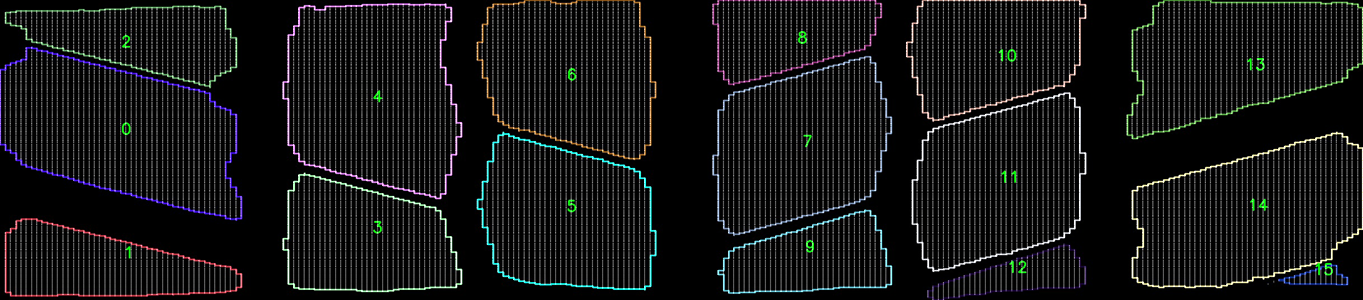
\includegraphics[width=0.9\columnwidth]{./pictures/batt_1a_analisi_b.png}
	\caption{Contorni dei Blob, in questo caso ne sono presenti 16.}\label{fig:batt_1a_analisi_b}
\end{figure}

\begin{figure}[H]
	\centering
	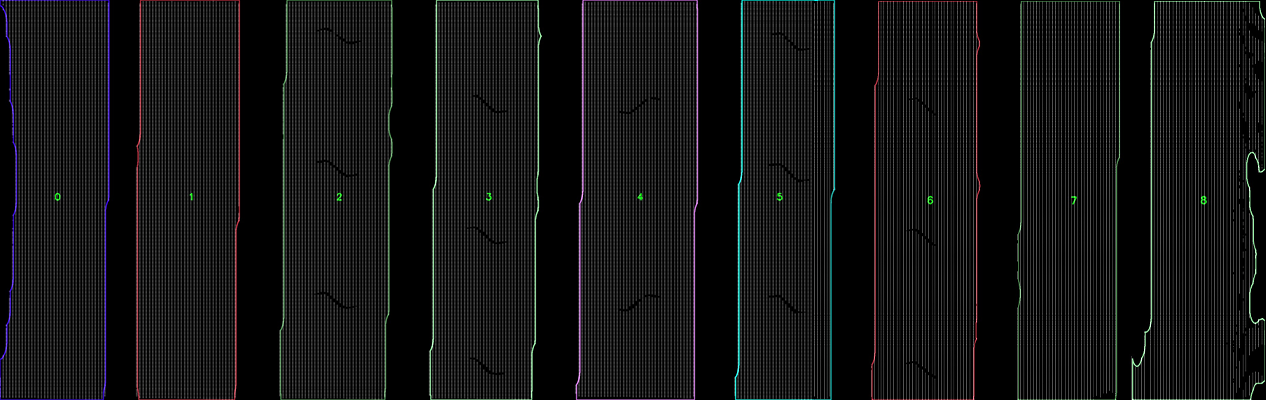
\includegraphics[width=0.9\columnwidth]{./pictures/batt_1b_analisi_mb.png}
	\caption{Contorni dei MacroBlob, in questo caso ne sono presenti 9.}\label{fig:batt_1b_analisi_mb}
\end{figure}

\noindent In seguito alla scansione dell'oggetto, da parte del profilometro laser, ciò che abbiamo non sono altro che delle coordinate \textit{x}, \textit{y} e \textit{z} dove sono definiti tutti i punti presenti nella \textit{point cloud}, dove il punto (0,0,0) coincide con il centro del piano della stessa (figura \ref{fig:batt_1a_analisi_1}).\\

\begin{figure}[H]
	\centering
	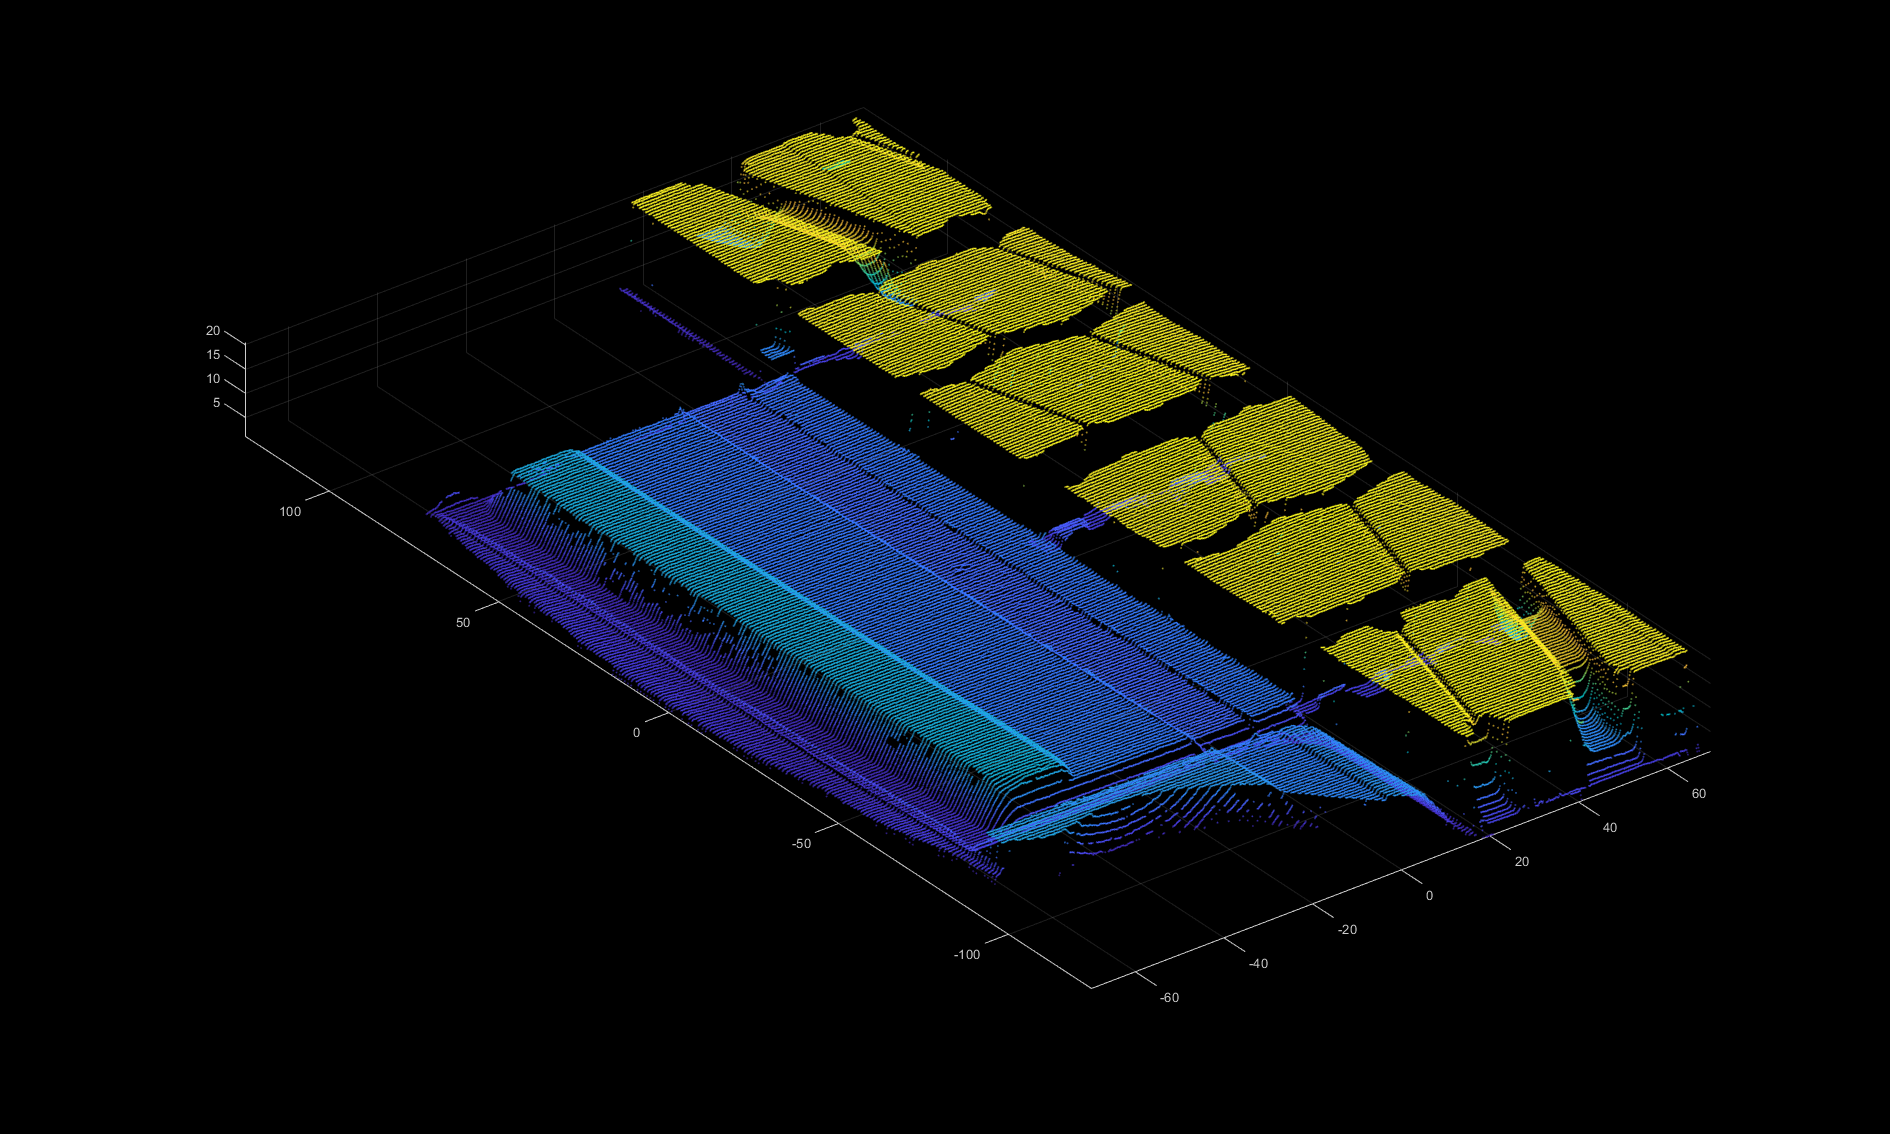
\includegraphics[width=0.8\columnwidth]{./pictures/batt_1a_analisi_1.png}
	\caption{Point cloud non elaborata del battistrada di tipo \textit{1A}.}\label{fig:batt_1a_analisi_1}
\end{figure}

\noindent La prima operazione effettuata è stata quella di applicare un filtro per rimuovere eventuali misurazioni rumorose, come ad esempio valori anomali. Infatti, le scansioni laser, generando \textit{point cloud} con una densità di punti variabile, effettuano spesso errori di misurazione che riportano valori anomali.\\
\newline
Per evitare il più possibile questi errori, è stata applicata un'analisi statistica sull'intorno di ciascun punto, filtrando quelli che non soddisfano un determinato criterio. Assumendo che la distribuzione risultante sia gaussiana con una media e una deviazione standard, tutti i punti le cui distanze medie sono al di fuori di un intervallo definito dalla media delle distanze globali e dalla deviazione standard, possono essere considerati valori anomali e quindi rimossi.\\
\newline
La figura \ref{fig:batt_1a_analisi_2} mostra gli effetti dell'analisi e della rimozione dei valori anomali.

\begin{figure}[H]
	\centering
	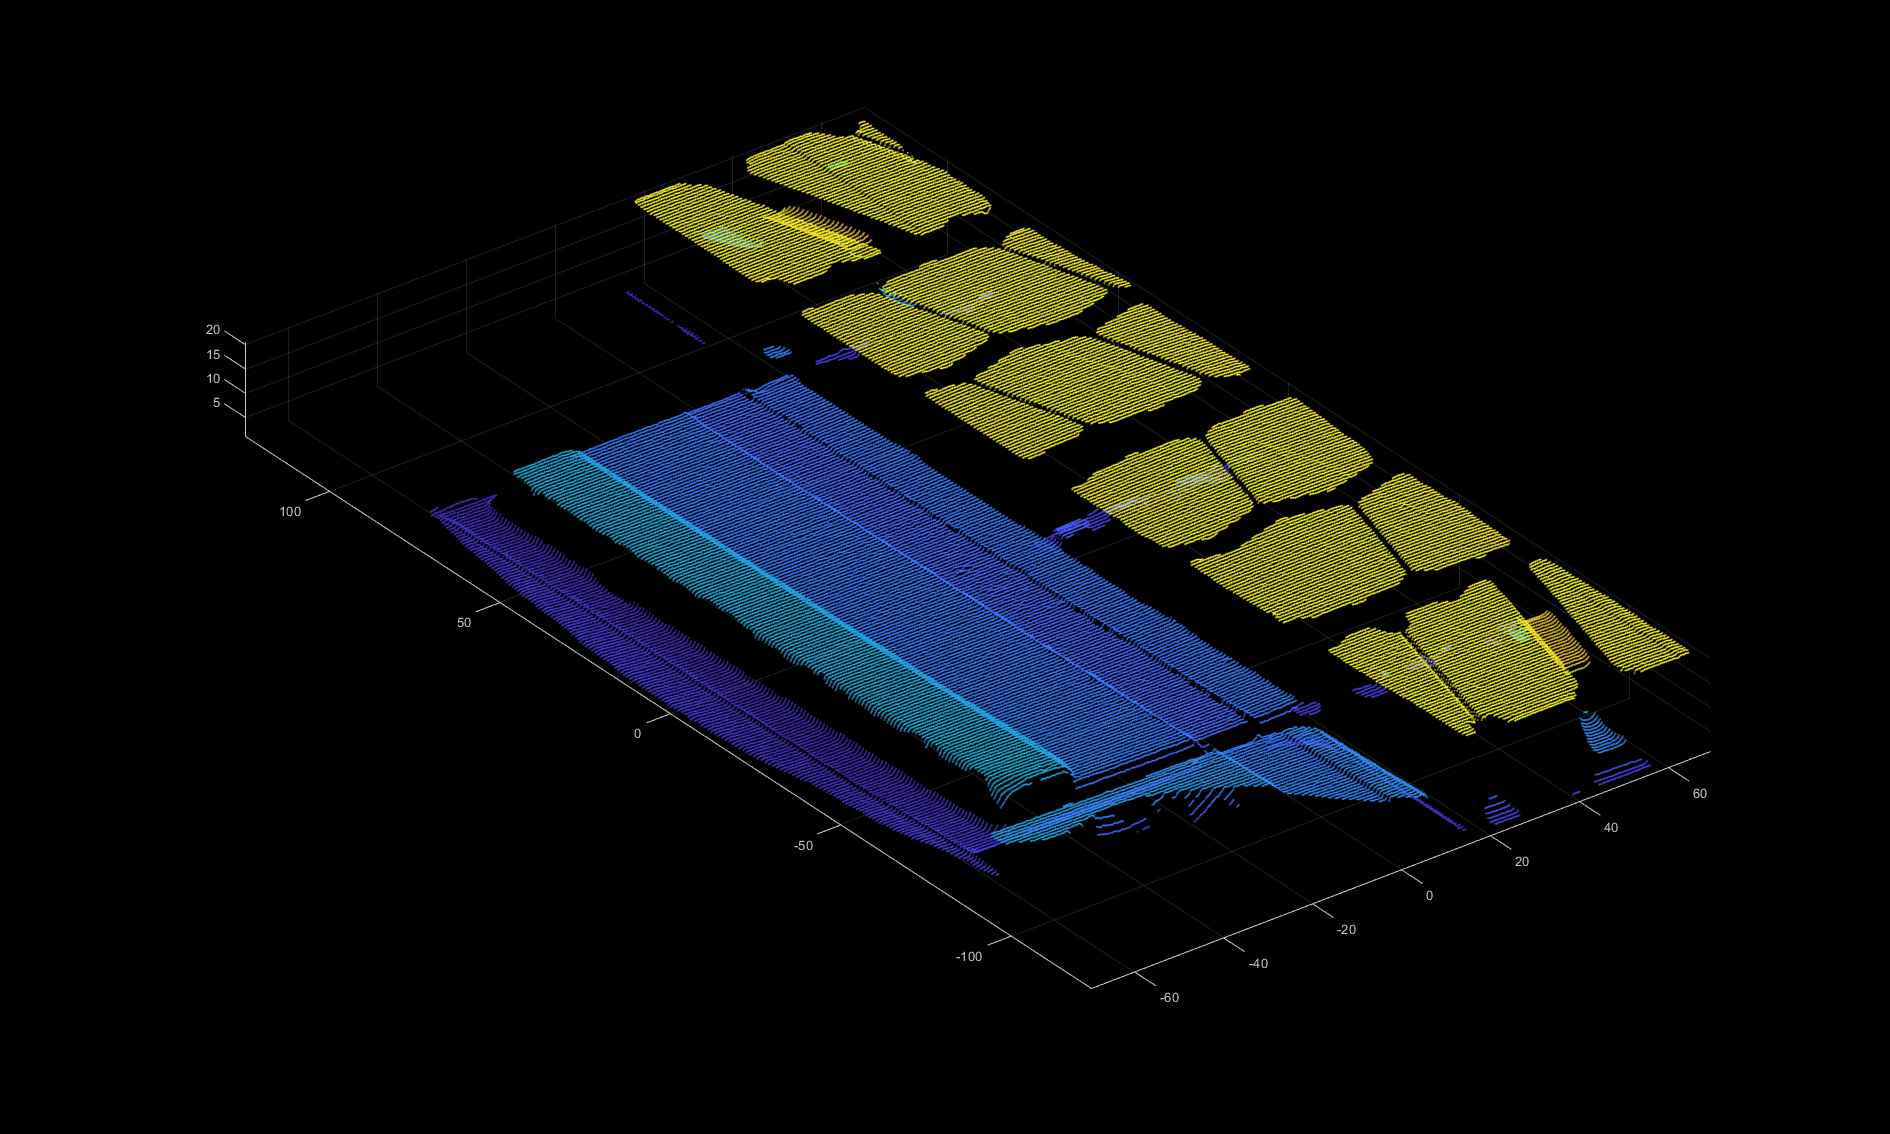
\includegraphics[width=0.8\columnwidth]{./pictures/batt_1a_analisi_2.png}
	\caption{Point cloud del battistrada di tipo \textit{1A} dopo aver applicato il filtro statistico.}\label{fig:batt_1a_analisi_2}
\end{figure}

\noindent Il nuovo obiettivo è quello di mascherare solo la parte dove si trovano i \textit{Blob} (punti di colore giallo della figura \ref{fig:batt_1a_analisi_2}). Per fare ciò, è stata eseguita una semplice segmentazione piana di un insieme di punti, ovvero sono stati trovati tutti i punti all'interno della nostra \textit{point cloud} che supportano un modello piano.\\
\newline
Dopo aver impostato il modello (\textit{pcl::SACMODEL\_PLANE}) e il tipo di metodo (\textit{pcl::SAC\_RANSAC}), è stata specificata una distanza di soglia che determina quanto un punto deve essere vicino al modello piano per essere considerato facente parte del modello stesso.\\
\newline
In questo caso è stata effettuata una prima distinzione tra il battistrada di tipo \textit{1A} e quello di tipo \textit{1B}, perchè sono state impostate diverse distanze di soglia per ognuno.

\begin{figure}[H]
	\centering
	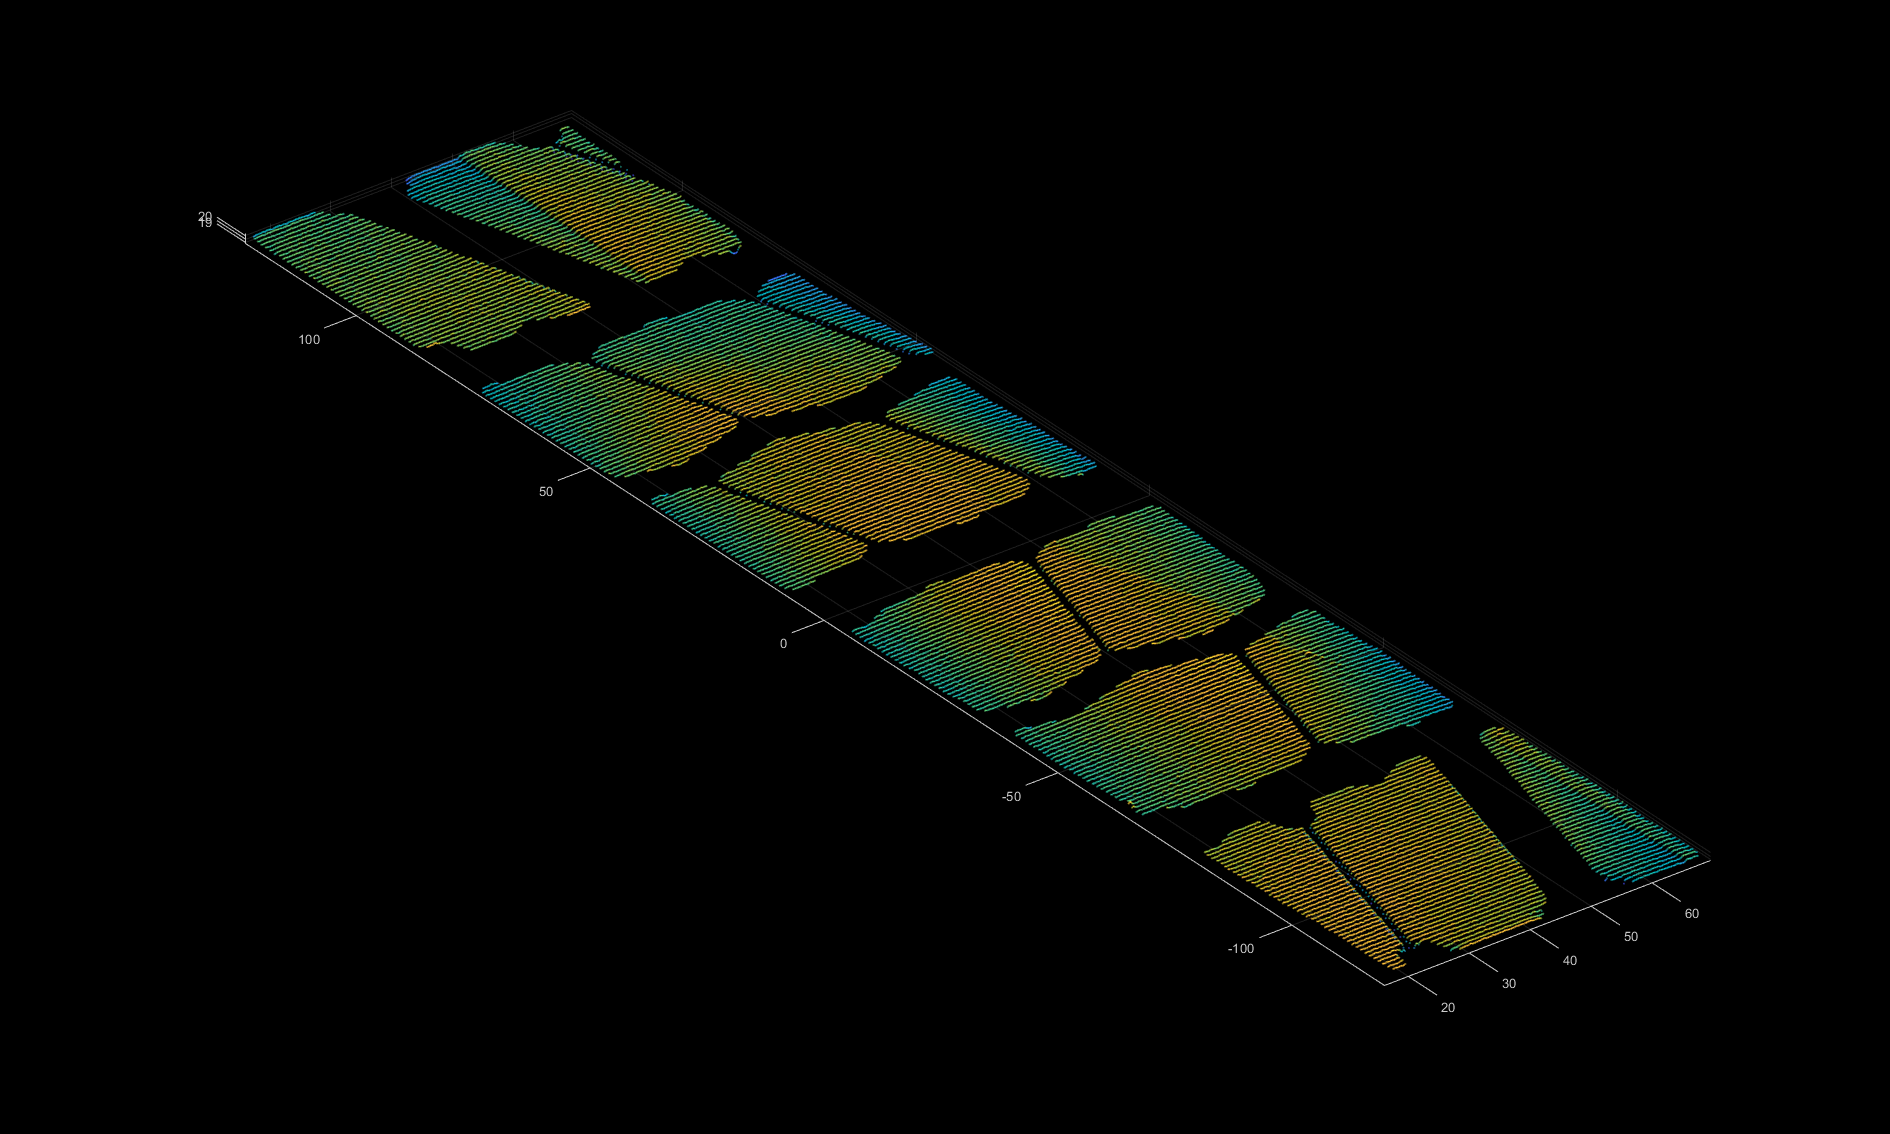
\includegraphics[width=0.8\columnwidth]{./pictures/batt_1a_analisi_3.png}
	\caption{Point cloud del battistrada di tipo \textit{1A} dopo aver applicato la segmentazione planare.}\label{fig:batt_1a_analisi_3}
\end{figure}

\noindent Le ultime due operazioni sulla \textit{point cloud} sono le più semplici. Prima, tutti i punti sono stati proiettati sul piano dato dalla sua equazione \textit{z = 0} (figura \ref{fig:batt_1a_analisi_4}), poi è stata effettuata un operazione di traslazione di tutti i punti portando l'origine degli assi nella posizione convenzionale di un immagine, in alto a sinistra (figura \ref{fig:batt_1a_analisi_5}).\\

\begin{figure}[H]
	\centering
	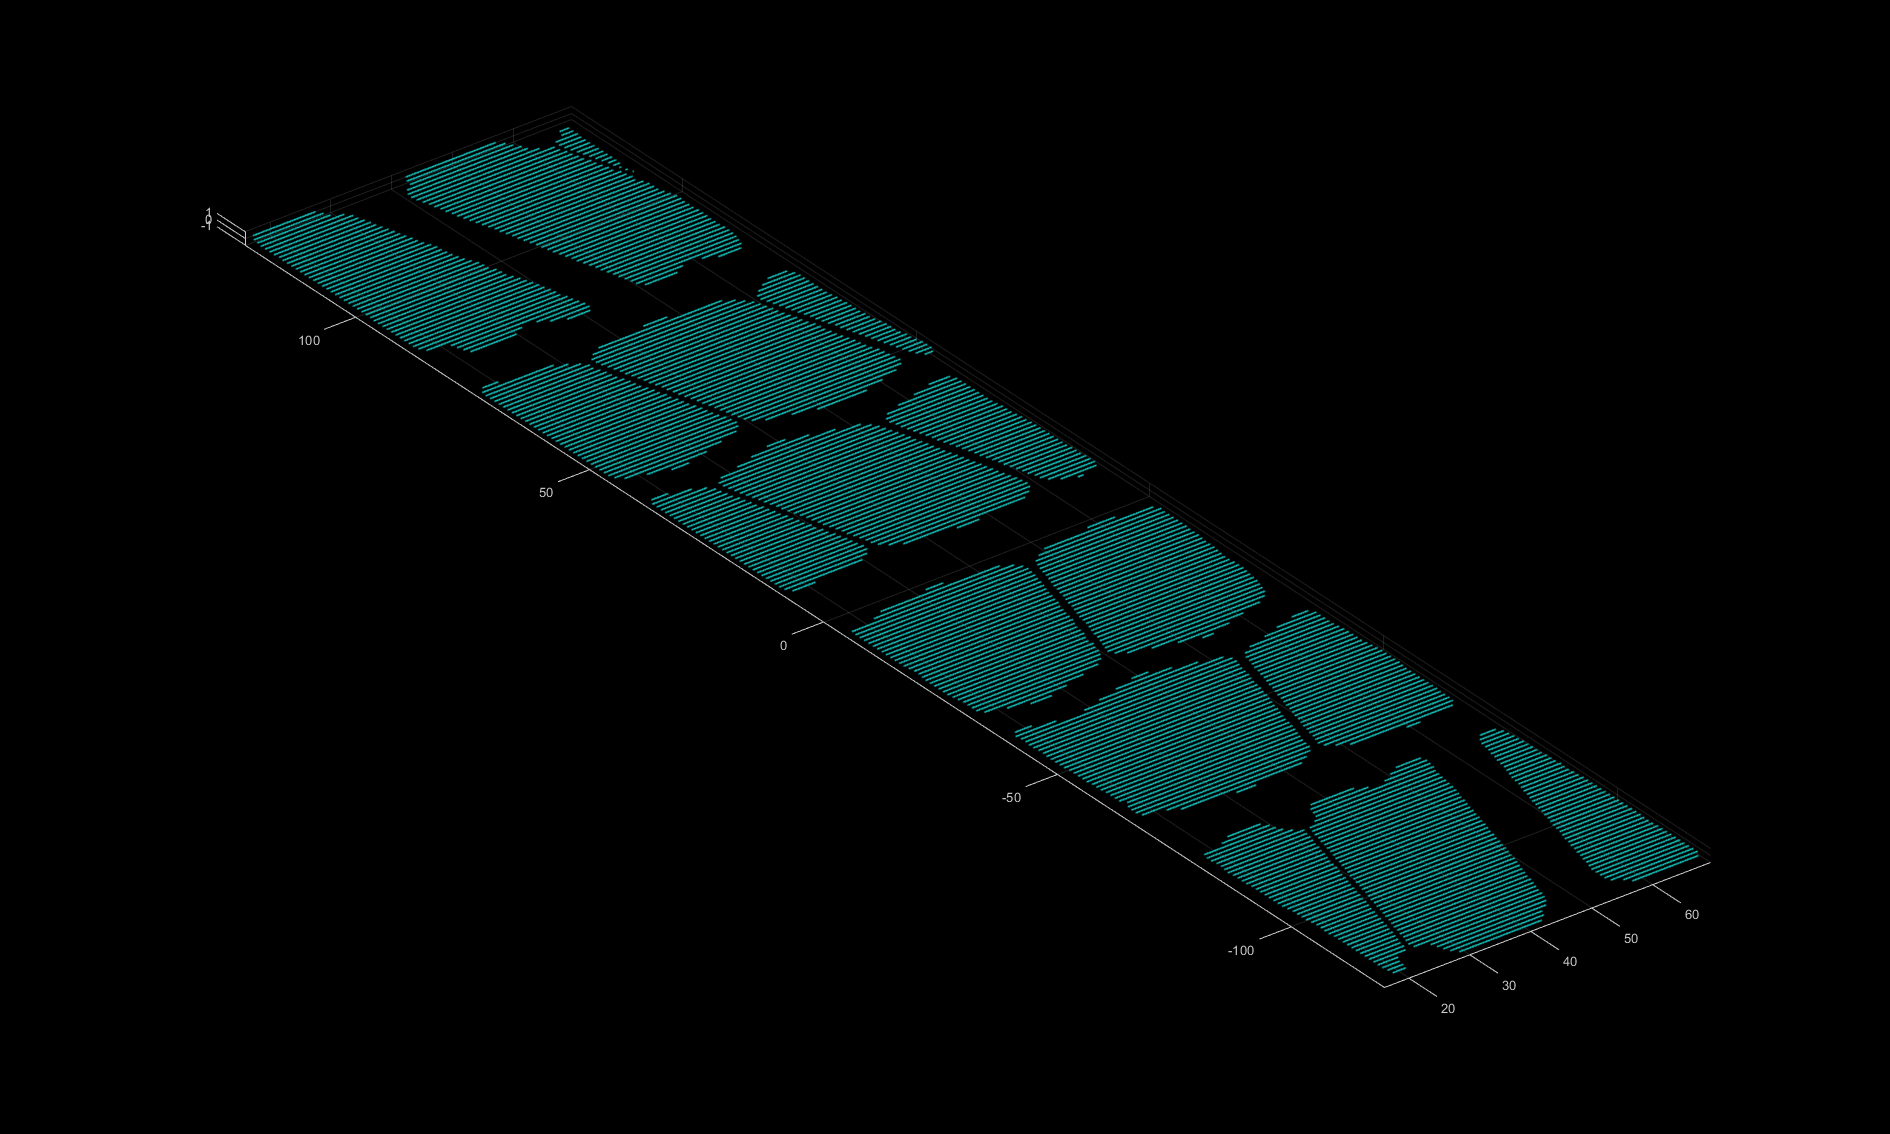
\includegraphics[width=0.8\columnwidth]{./pictures/batt_1a_analisi_4.png}
	\caption{Point cloud del battistrada di tipo \textit{1A} dopo aver applicato l'operazione di proiezione.}\label{fig:batt_1a_analisi_4}
\end{figure}

\begin{figure}[H]
	\centering
	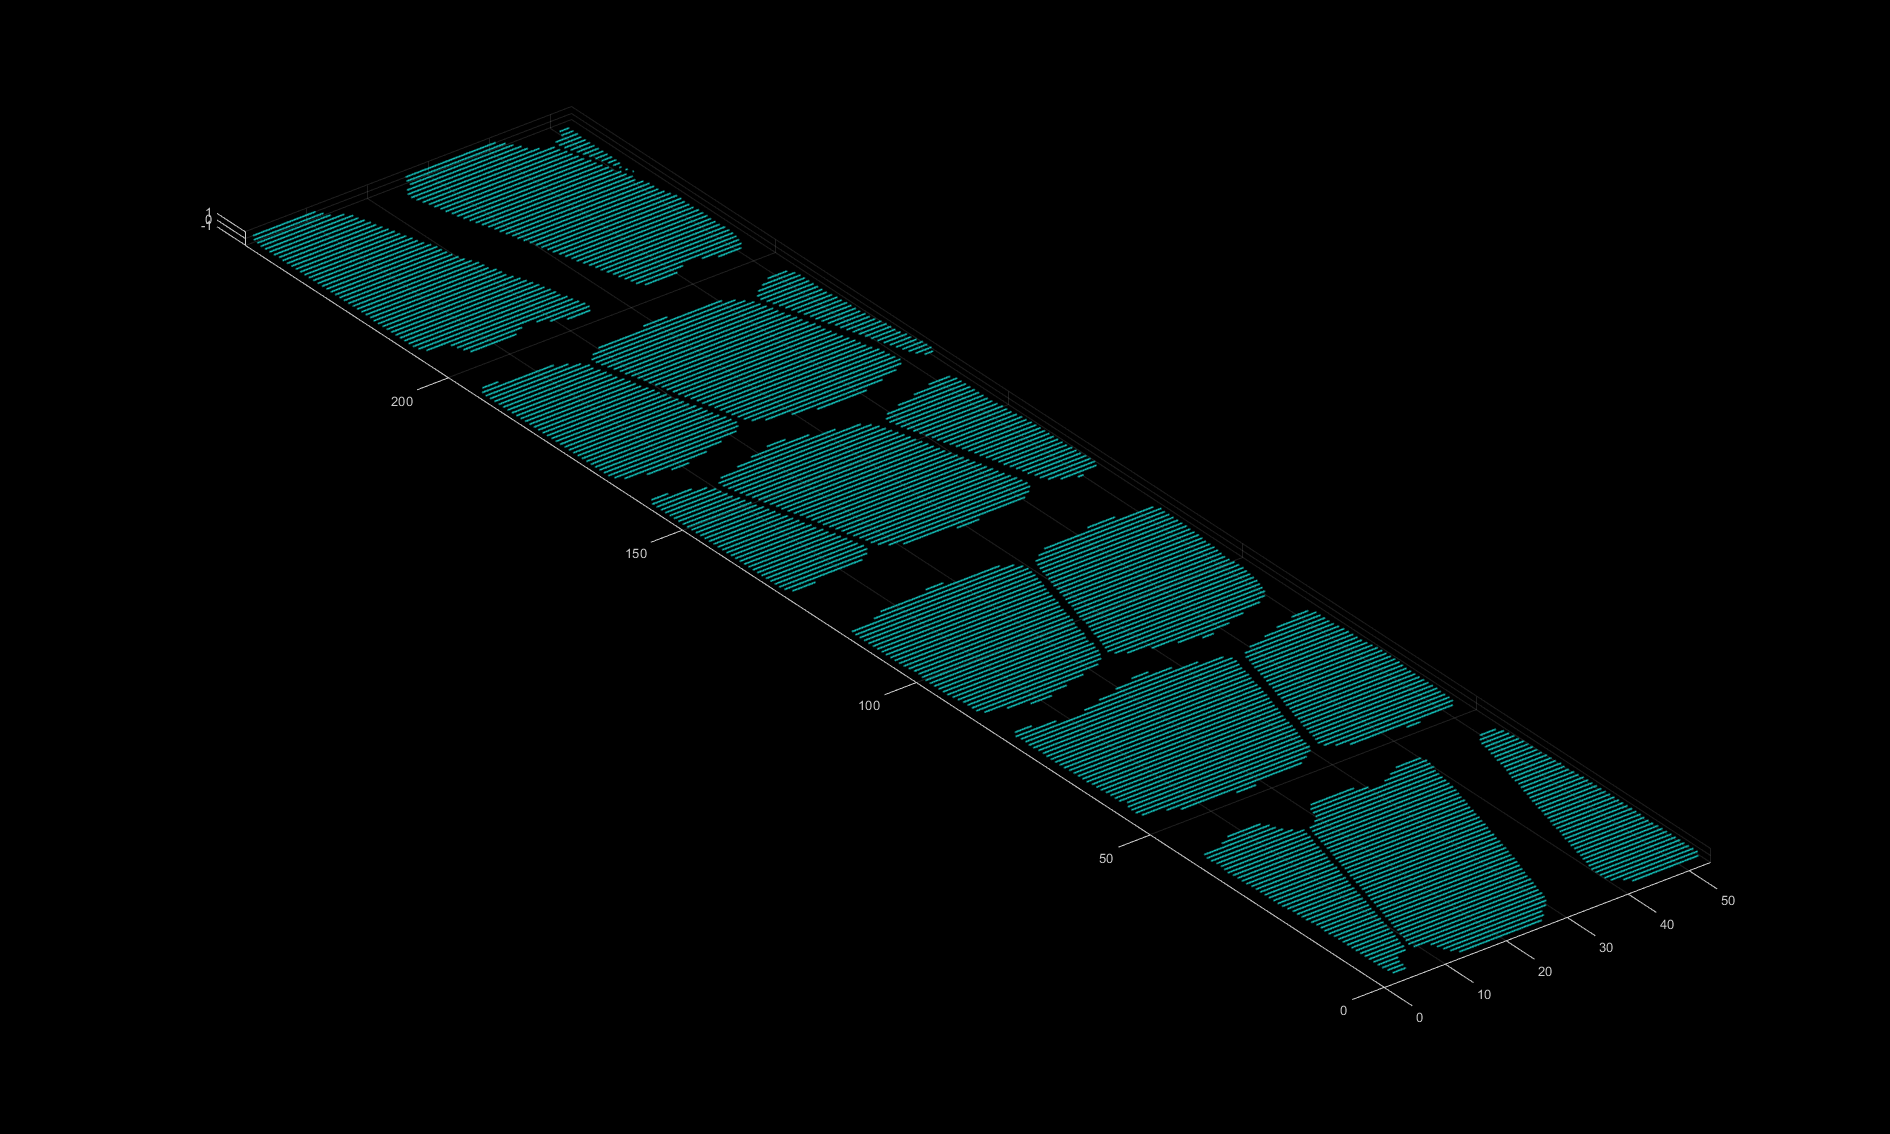
\includegraphics[width=0.8\columnwidth]{./pictures/batt_1a_analisi_5.png}
	\caption{Point cloud del battistrada di tipo \textit{1A} dopo aver applicato l'operazione di traslazione.}\label{fig:batt_1a_analisi_5}
\end{figure}

\noindent A questo punto, per trovare i contorni e le misure dei vari blocchi, si è deciso di utilizzare la libreria \textit{opencv} e quindi è stato necessario creare un immagine dove i punti della \textit{point cloud} sono stati colorati di bianco e tutto il resto di nero.\\
Inoltre è stato applicato un moltiplicatore x10 cosicché 1 pixel dell'immagine corrispondesse, nel mondo reale, ad 1 µm.\\

\begin{figure}[H]
	\centering
	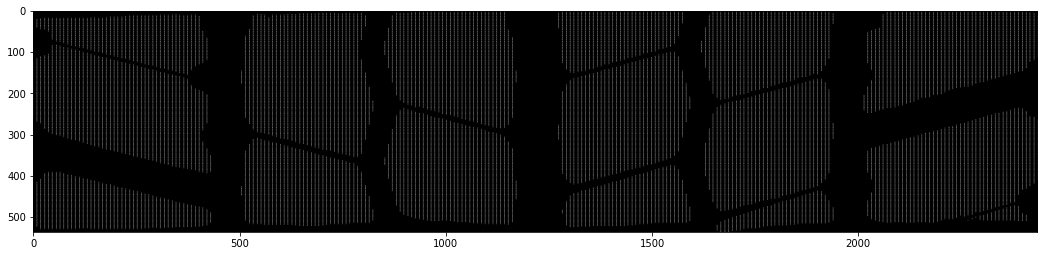
\includegraphics[width=0.9\columnwidth]{./pictures/batt_1a_analisi_6.png}
	\caption{Immagine planare del battistrada di tipo \textit{1A}.}\label{fig:batt_1a_analisi_6}
\end{figure}

\noindent Per chiudere i piccoli fori presenti nei \textit{Blob} della figura \ref{fig:batt_1a_analisi_6}, sono state usate delle trasformazioni morfologiche, in particolare di tipo \textit{closing}.\\
\newline
Le trasformazioni morfologiche sono delle operazioni che si basano sulla forma dell'immagine. L'operazione di tipo \textit{closing} non è altro che il susseguirsi di due operatori: prima viene applicata una \textit{dilatazione} e poi un \textit{erosione}.\\
La figura \ref{fig:batt_1a_analisi_7} è il risultato della prima \textit{closing} applicata per trovare i \textit{Blob}, mentre la figura \ref{fig:batt_1a_analisi_8} è il risultato della \textit{closing} applicata all'immagine precedente per trovare i \textit{MacroBlob}.\\

\begin{figure}[H]
	\centering
	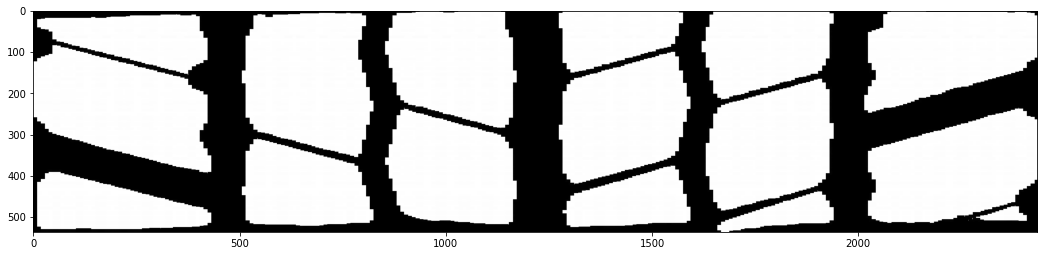
\includegraphics[width=0.9\columnwidth]{./pictures/batt_1a_analisi_7.png}
	\caption{Immagine del battistrada di tipo \textit{1A} dopo aver applicato la prima trasformazione morfologica (Closing).}\label{fig:batt_1a_analisi_7}
\end{figure}

\begin{figure}[H]
	\centering
	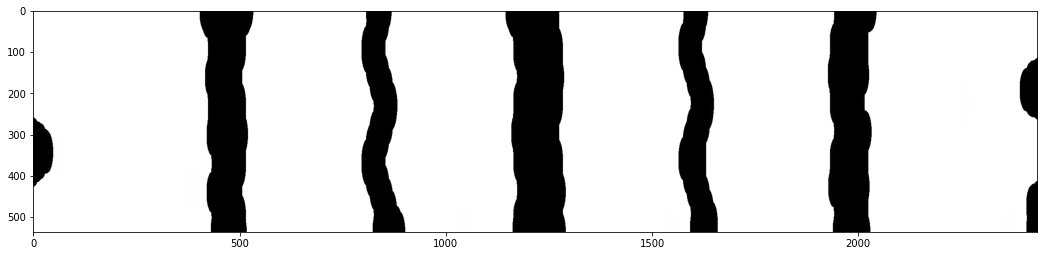
\includegraphics[width=0.9\columnwidth]{./pictures/batt_1a_analisi_8.png}
	\caption{Immagine del battistrada di tipo \textit{1A} dopo aver applicato la seconda trasformazione morfologica (Closing).}\label{fig:batt_1a_analisi_8}
\end{figure}

\noindent Quindi per trovare i contorni è stata utilizzata la funzione \textit{findContours()} di \textit{opencv} che accetta come argomenti: l'immagine sorgente in scala di grigio, la modalità di recupero (\textit{cv::RETR\_EXTERNAL}) e il metodo di approssimazione (\textit{cv::CHAIN\_APPROX\_NONE}) del contorno.\\
\newline
Una volta trovate tutte le coordinate dei punti dei contorni, è risultato immediato calcolare area (\textit{cv::contourArea()}) e perimetro (\textit{cv::arcLength()}). Per quanto riguarda le altre misure, si è preferito ricavarle dalle \textit{bounding box} di ogni blocco come si può vedere nelle figure \ref{fig:batt_1a_analisi_10} e \ref{fig:batt_1a_analisi_12}.\\
\newline
Per distinguere il battistrada di tipo \textit{1A} da quello di tipo \textit{1B}, è stata inserita, nel codice, la condizione che se il numero di \textit{Blob} e \textit{MacroBlob} trovati fosse uguale allora non si prosegue nel trovare la distanza minima tra \textit{Blob} in quanto sarebbe uguale a quella tra \textit{MacroBlob}.

\begin{figure}[H]
	\centering
	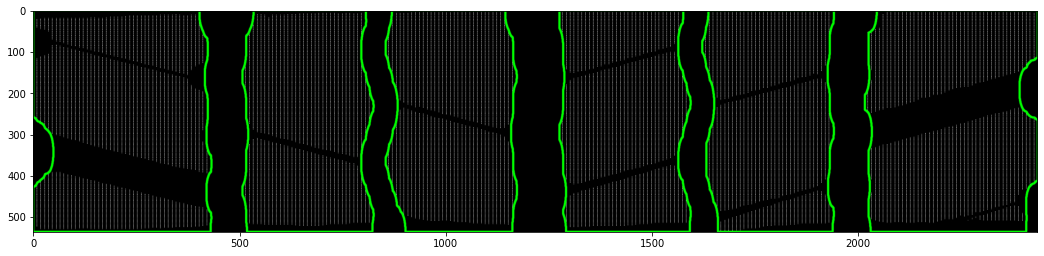
\includegraphics[width=0.9\columnwidth]{./pictures/batt_1a_analisi_9.png}
	\caption{Immagine del battistrada di tipo \textit{1A} con i contorni dei MacroBlob evidenziati.}\label{fig:batt_1a_analisi_9}
\end{figure}

\begin{figure}[H]
	\centering
	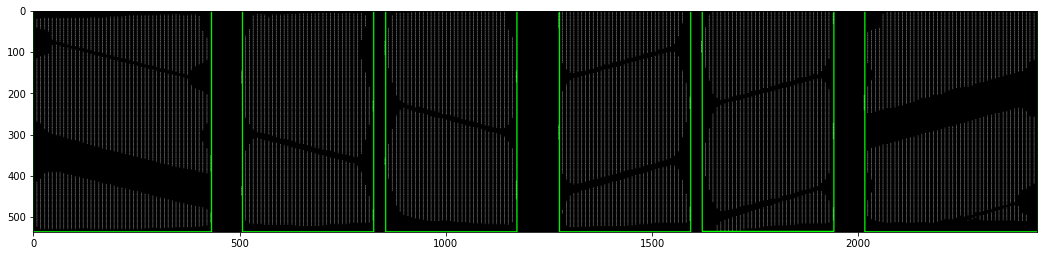
\includegraphics[width=0.9\columnwidth]{./pictures/batt_1a_analisi_10.png}
	\caption{Immagine del battistrada di tipo \textit{1A} con le bounding box dei MacroBlob evidenziate.}\label{fig:batt_1a_analisi_10}
\end{figure}

\begin{figure}[H]
	\centering
	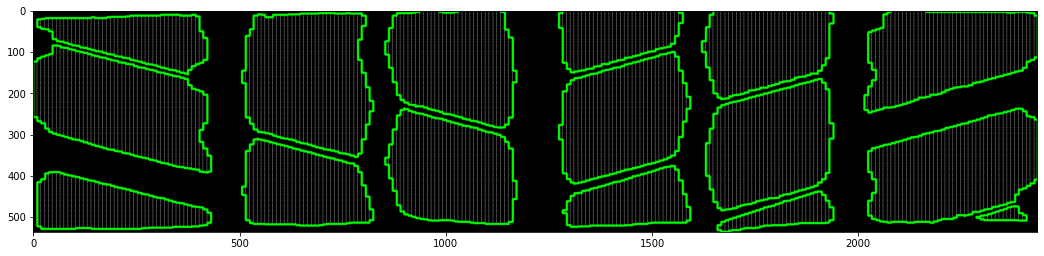
\includegraphics[width=0.9\columnwidth]{./pictures/batt_1a_analisi_11.png}
	\caption{Immagine del battistrada di tipo \textit{1A} con i contorni dei Blob evidenziati.}\label{fig:batt_1a_analisi_11}
\end{figure}

\begin{figure}[H]
	\centering
	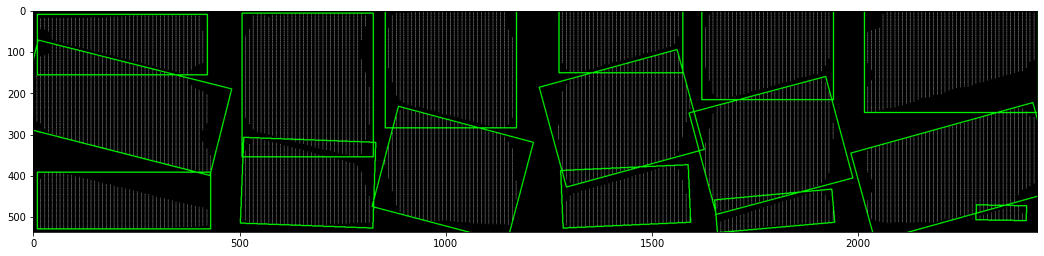
\includegraphics[width=0.9\columnwidth]{./pictures/batt_1a_analisi_12.png}
	\caption{Immagine del battistrada di tipo \textit{1A} con le bounding box dei Blob evidenziate.}\label{fig:batt_1a_analisi_12}
\end{figure}

\noindent Per trovare la distanza minima tra \textit{Blob} adiacenti presenti in ogni \textit{MacroBlob} è stata creata una funzione specifica che confronta le varie distanze tra i centri dei \textit{Blob}.

% \cppexternal{./codes/f.cpp}

\noindent Di seguito vengono illustrati i passaggi seguiti per il battistrada di tipo \textit{1B}.\\

\begin{figure}[H]
	\centering
	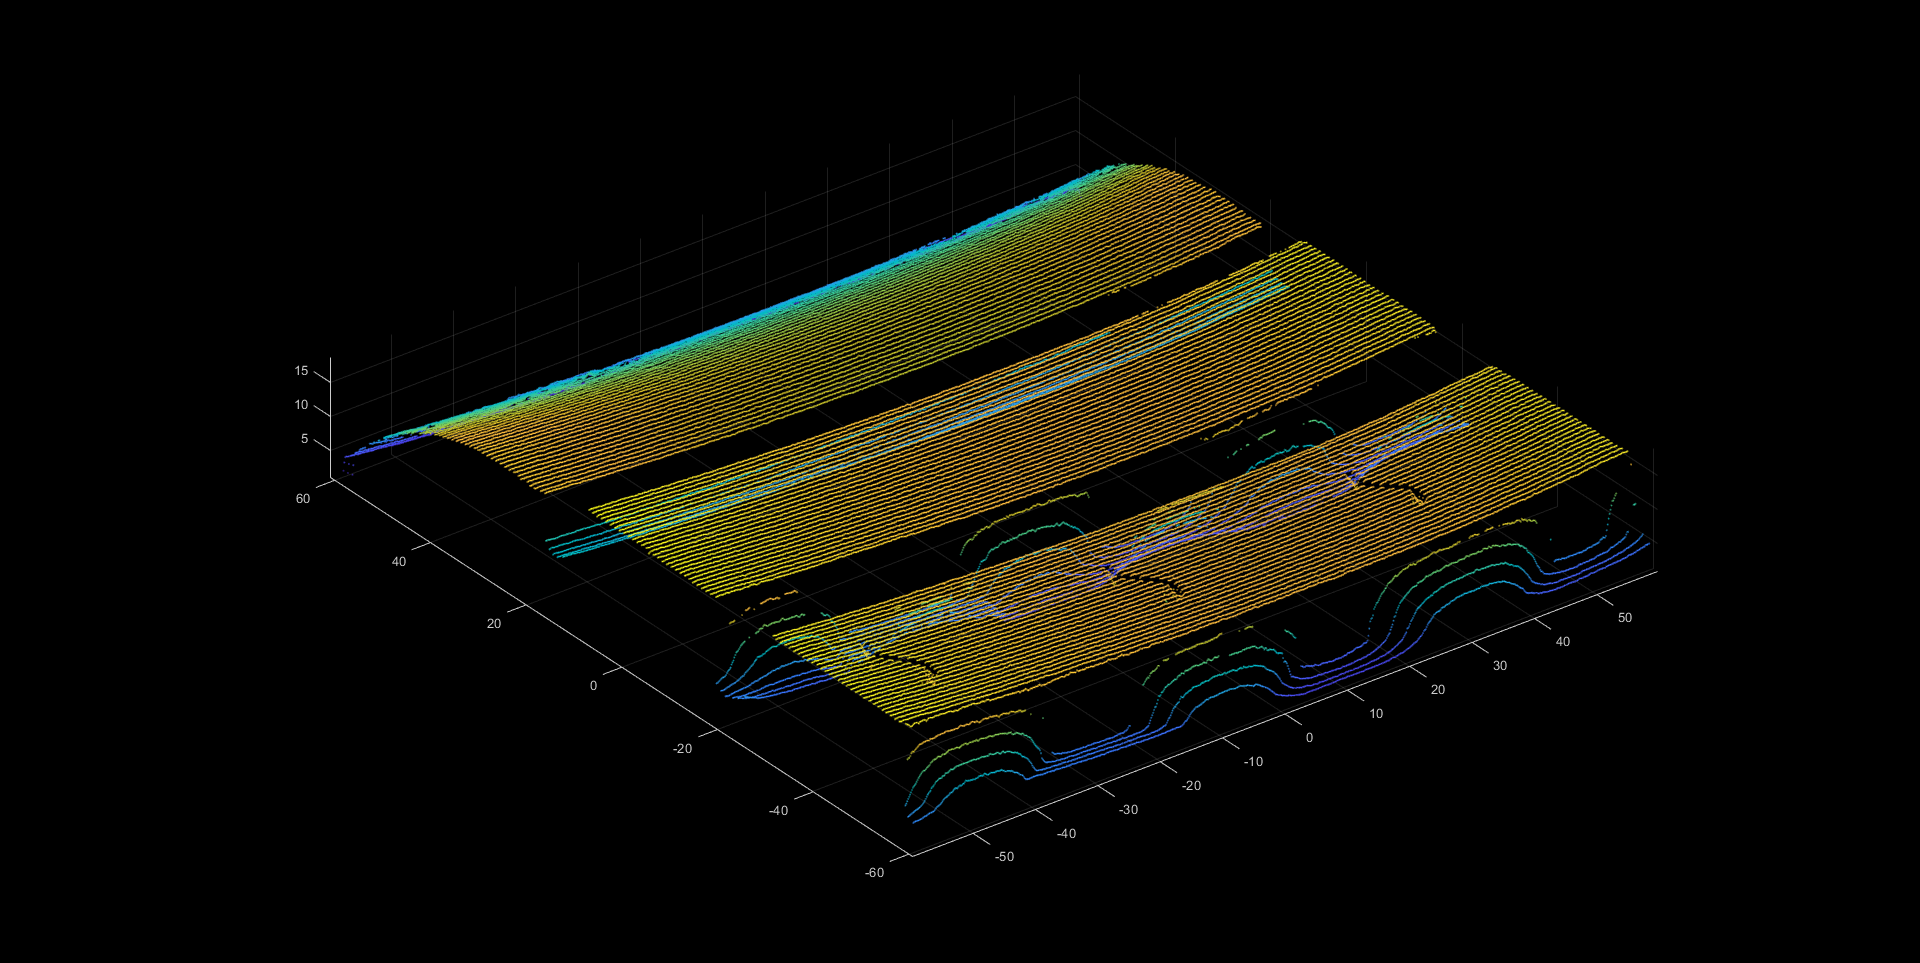
\includegraphics[width=0.45\columnwidth]{./pictures/batt_1b_analisi_1_1.png}
	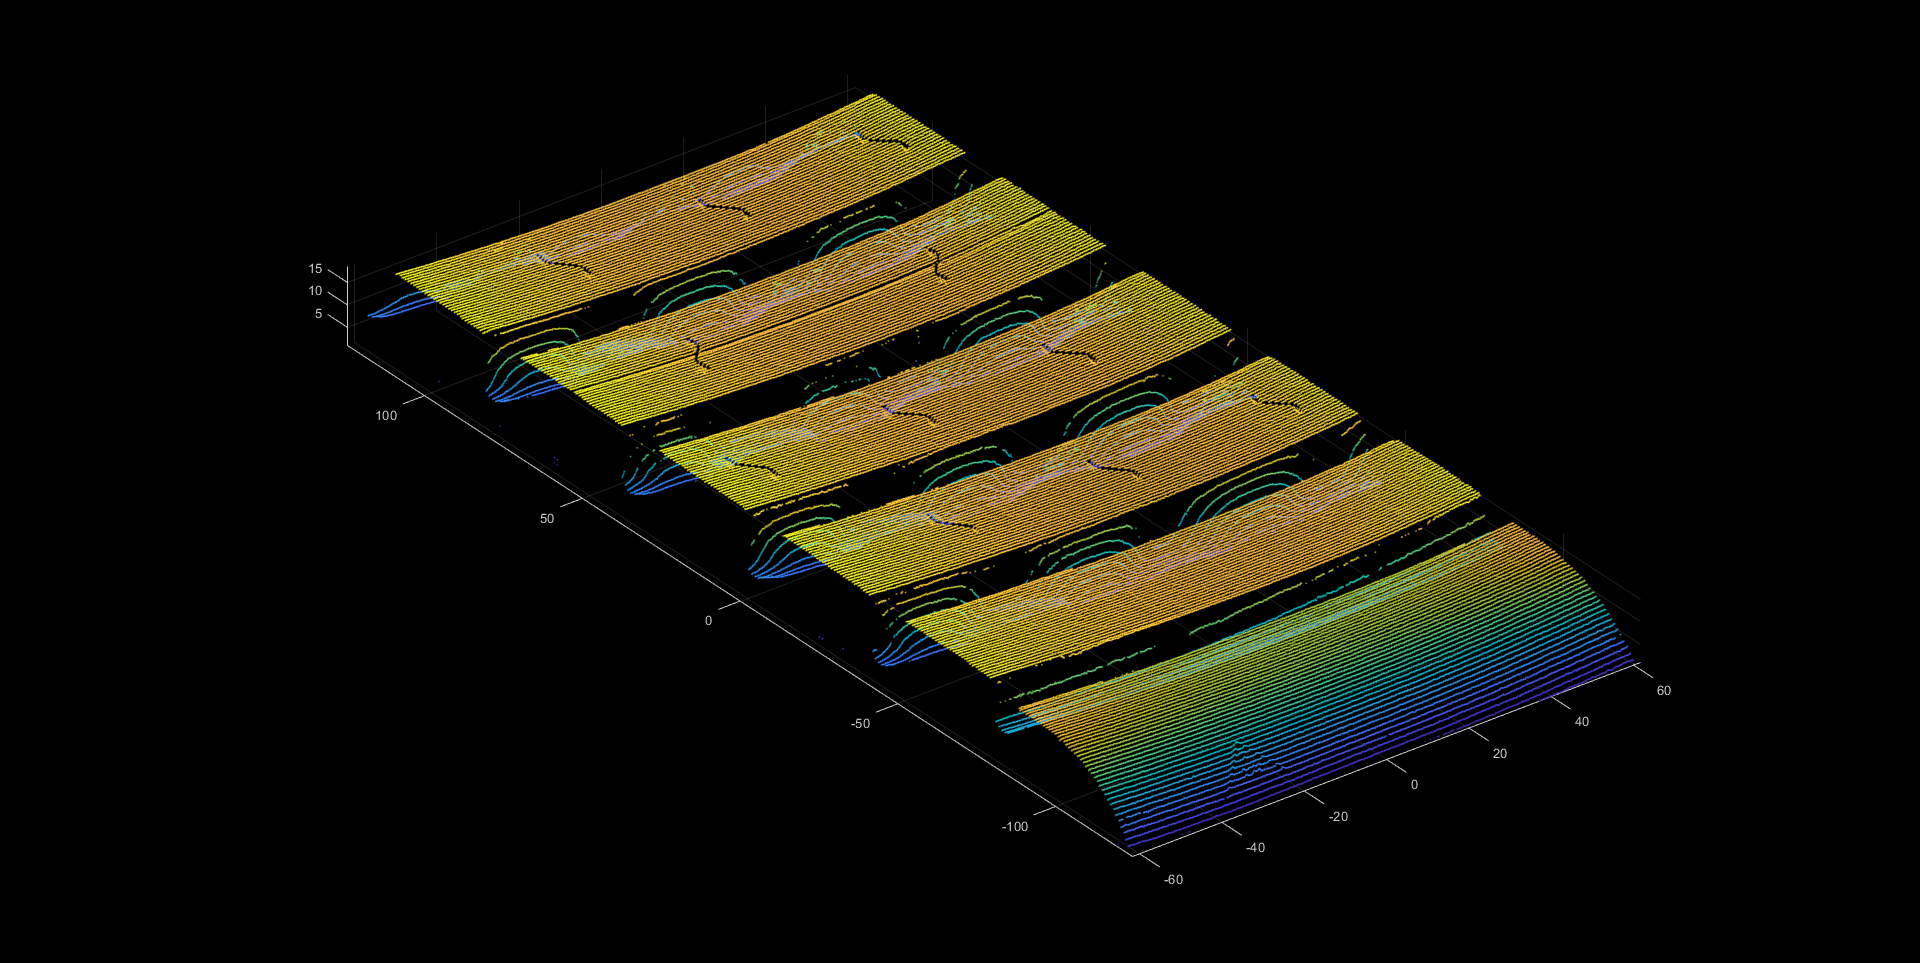
\includegraphics[width=0.45\columnwidth]{./pictures/batt_1b_analisi_2_1.png}
	\caption{Point cloud non elaborata del battistrada di tipo \textit{1B}.}\label{fig:batt_1b_analisi_1}
\end{figure}

\begin{figure}[H]
	\centering
	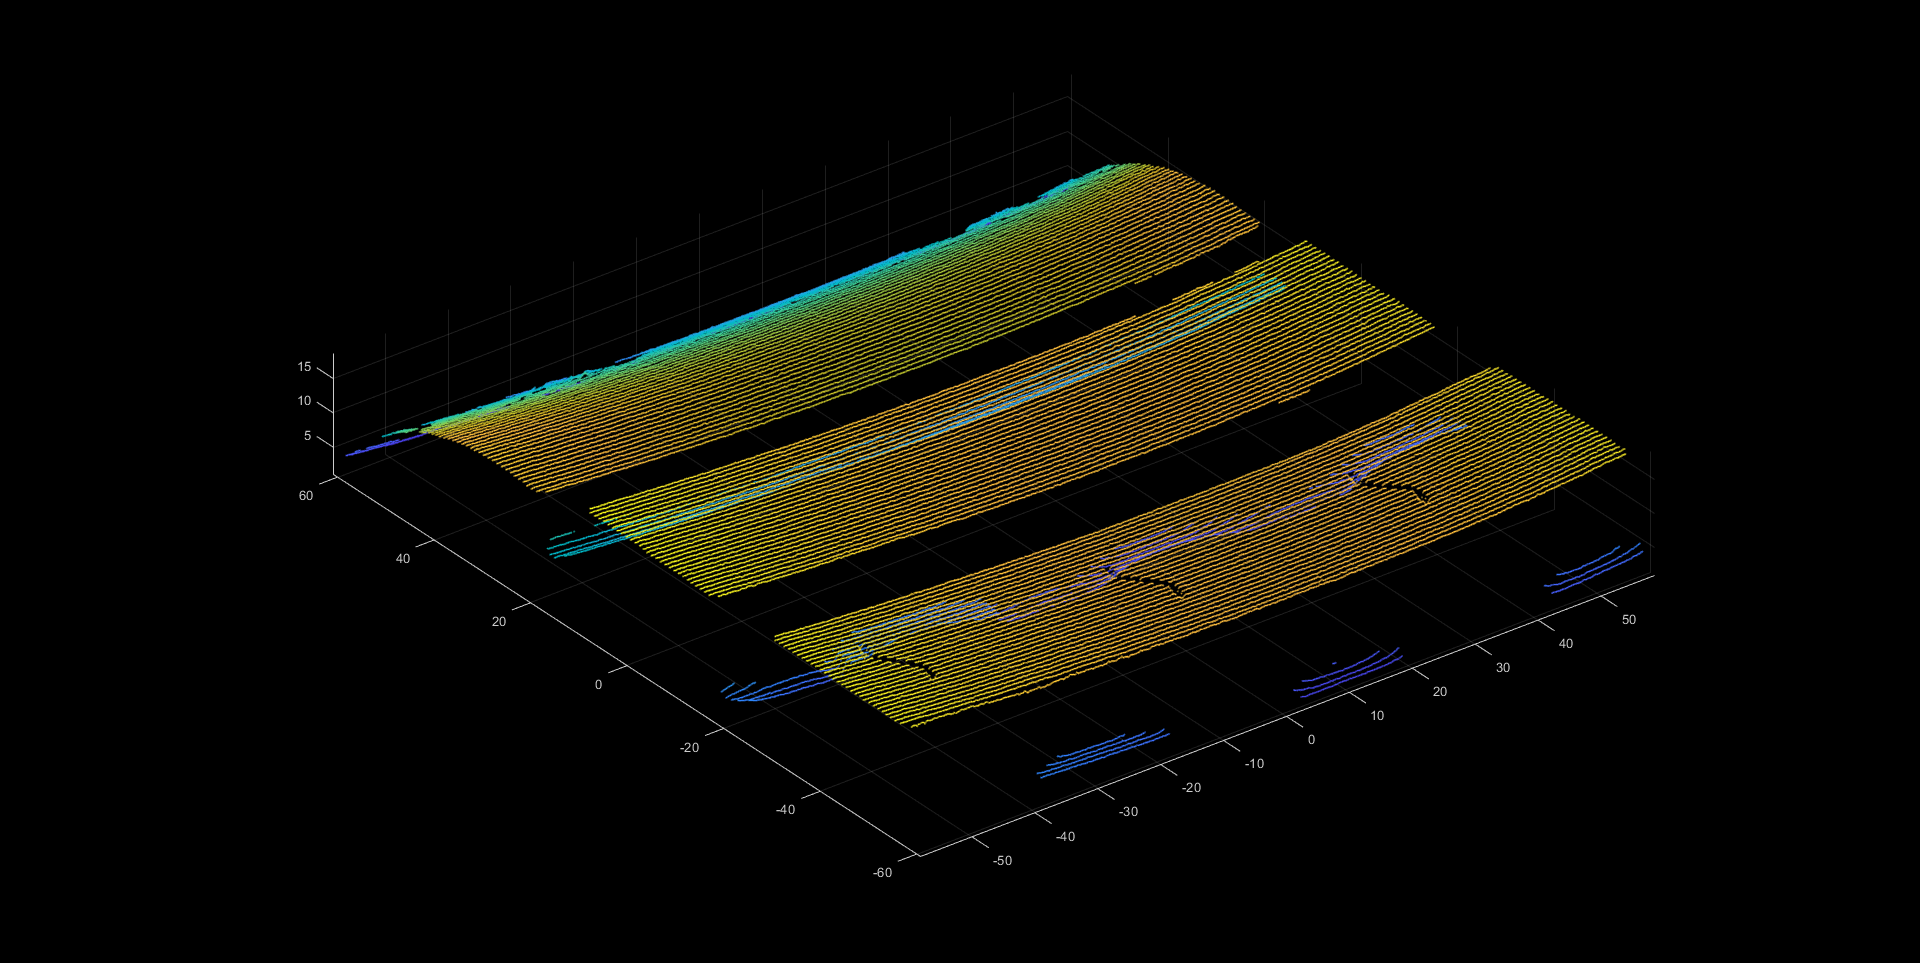
\includegraphics[width=0.45\columnwidth]{./pictures/batt_1b_analisi_1_2.png}
	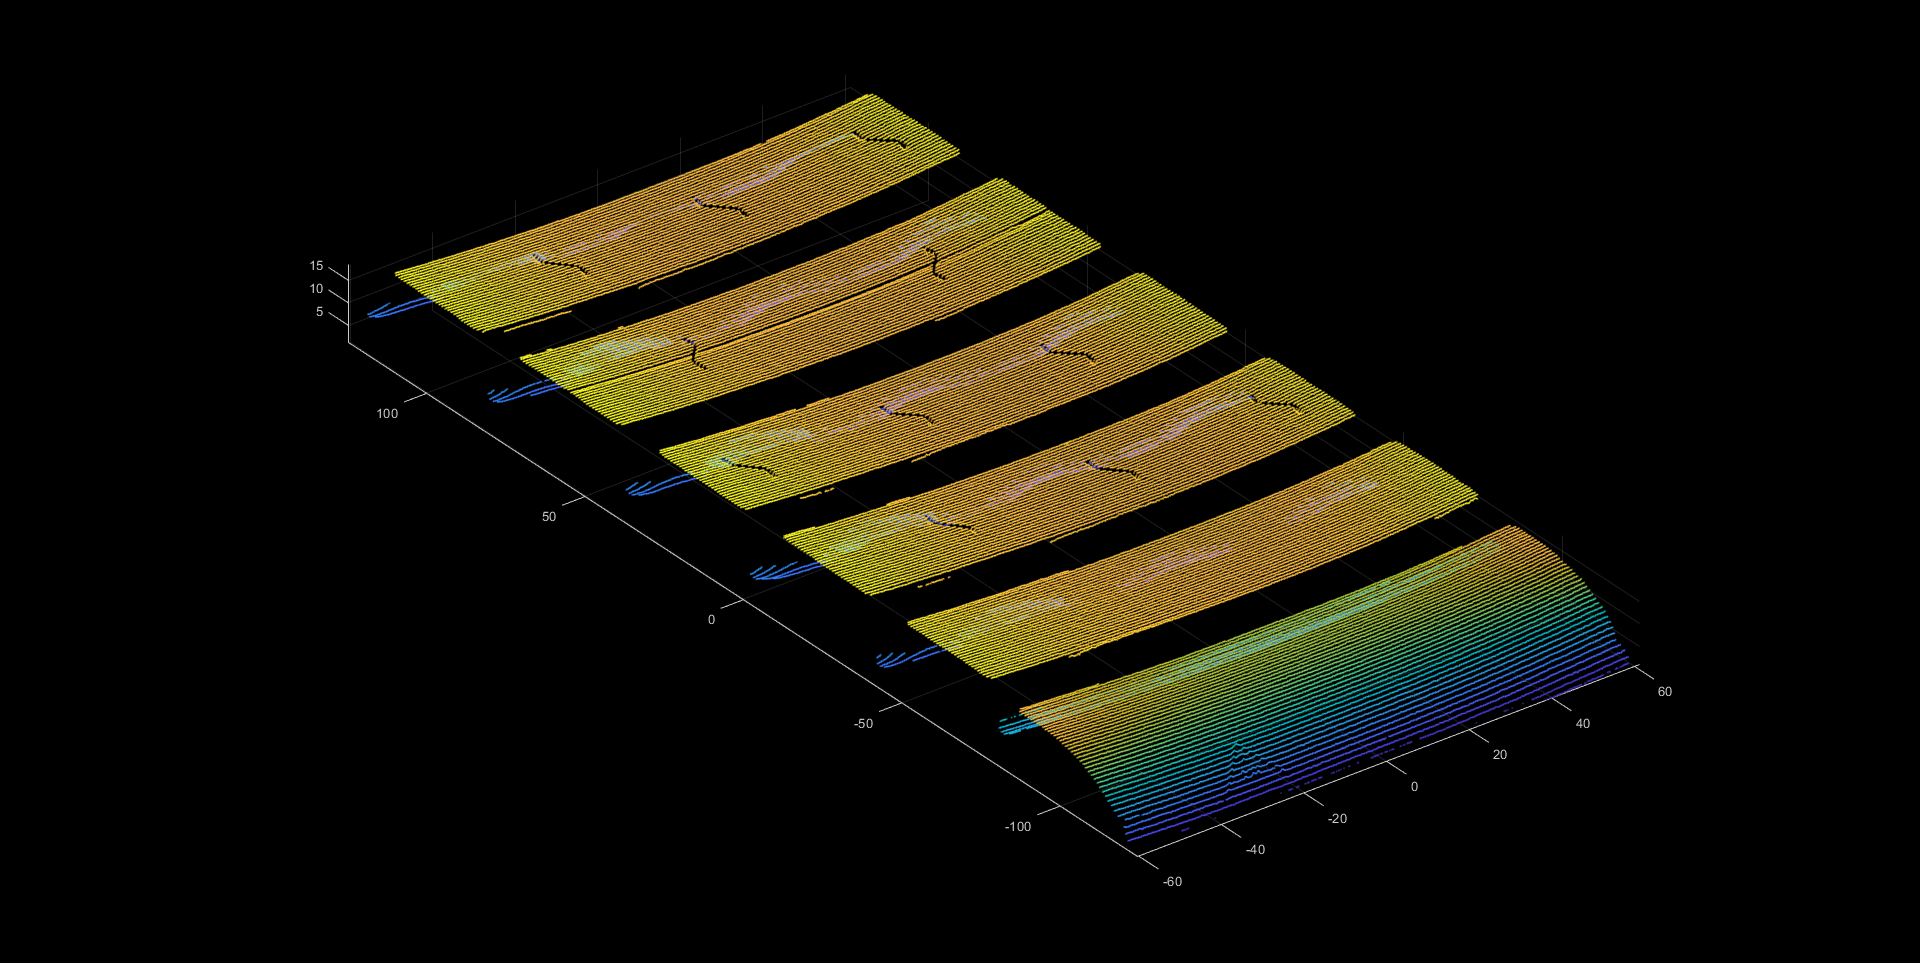
\includegraphics[width=0.45\columnwidth]{./pictures/batt_1b_analisi_2_2.png}
	\caption{Point cloud del battistrada di tipo \textit{1B} dopo aver applicato il filtro statistico.}\label{fig:batt_1b_analisi_2}
\end{figure}

\begin{figure}[H]
	\centering
	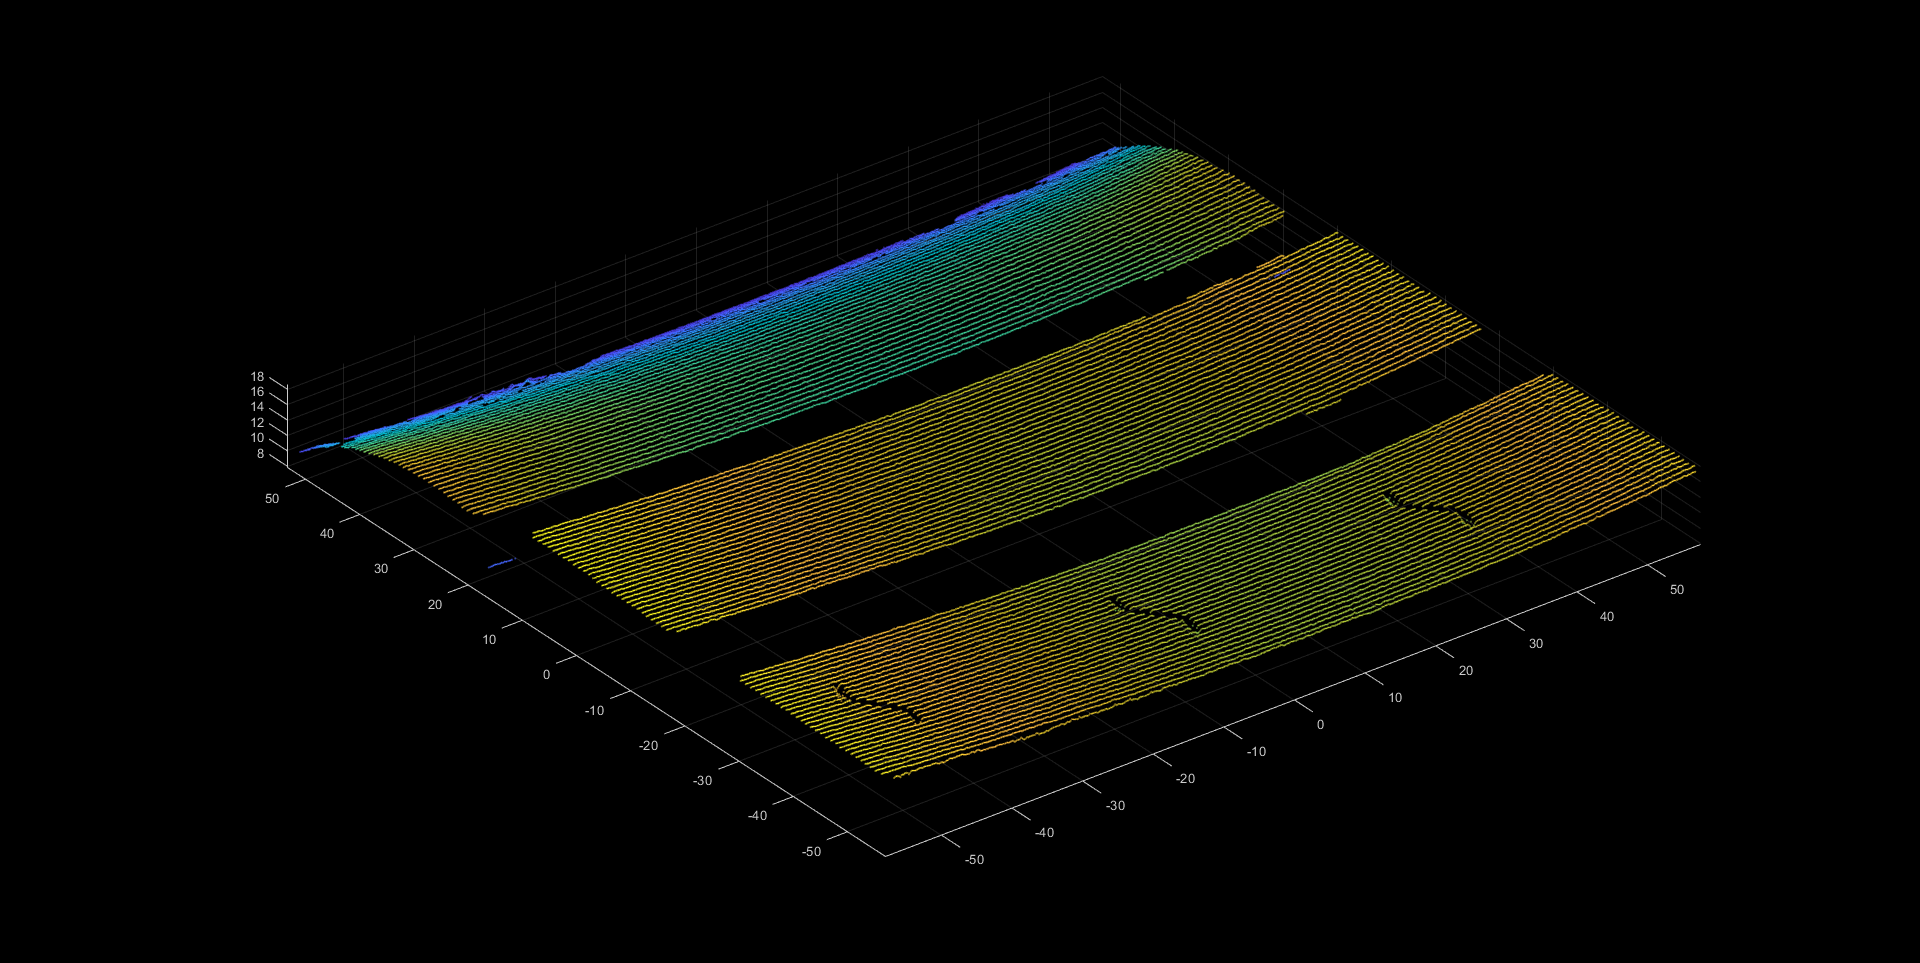
\includegraphics[width=0.45\columnwidth]{./pictures/batt_1b_analisi_1_3.png}
	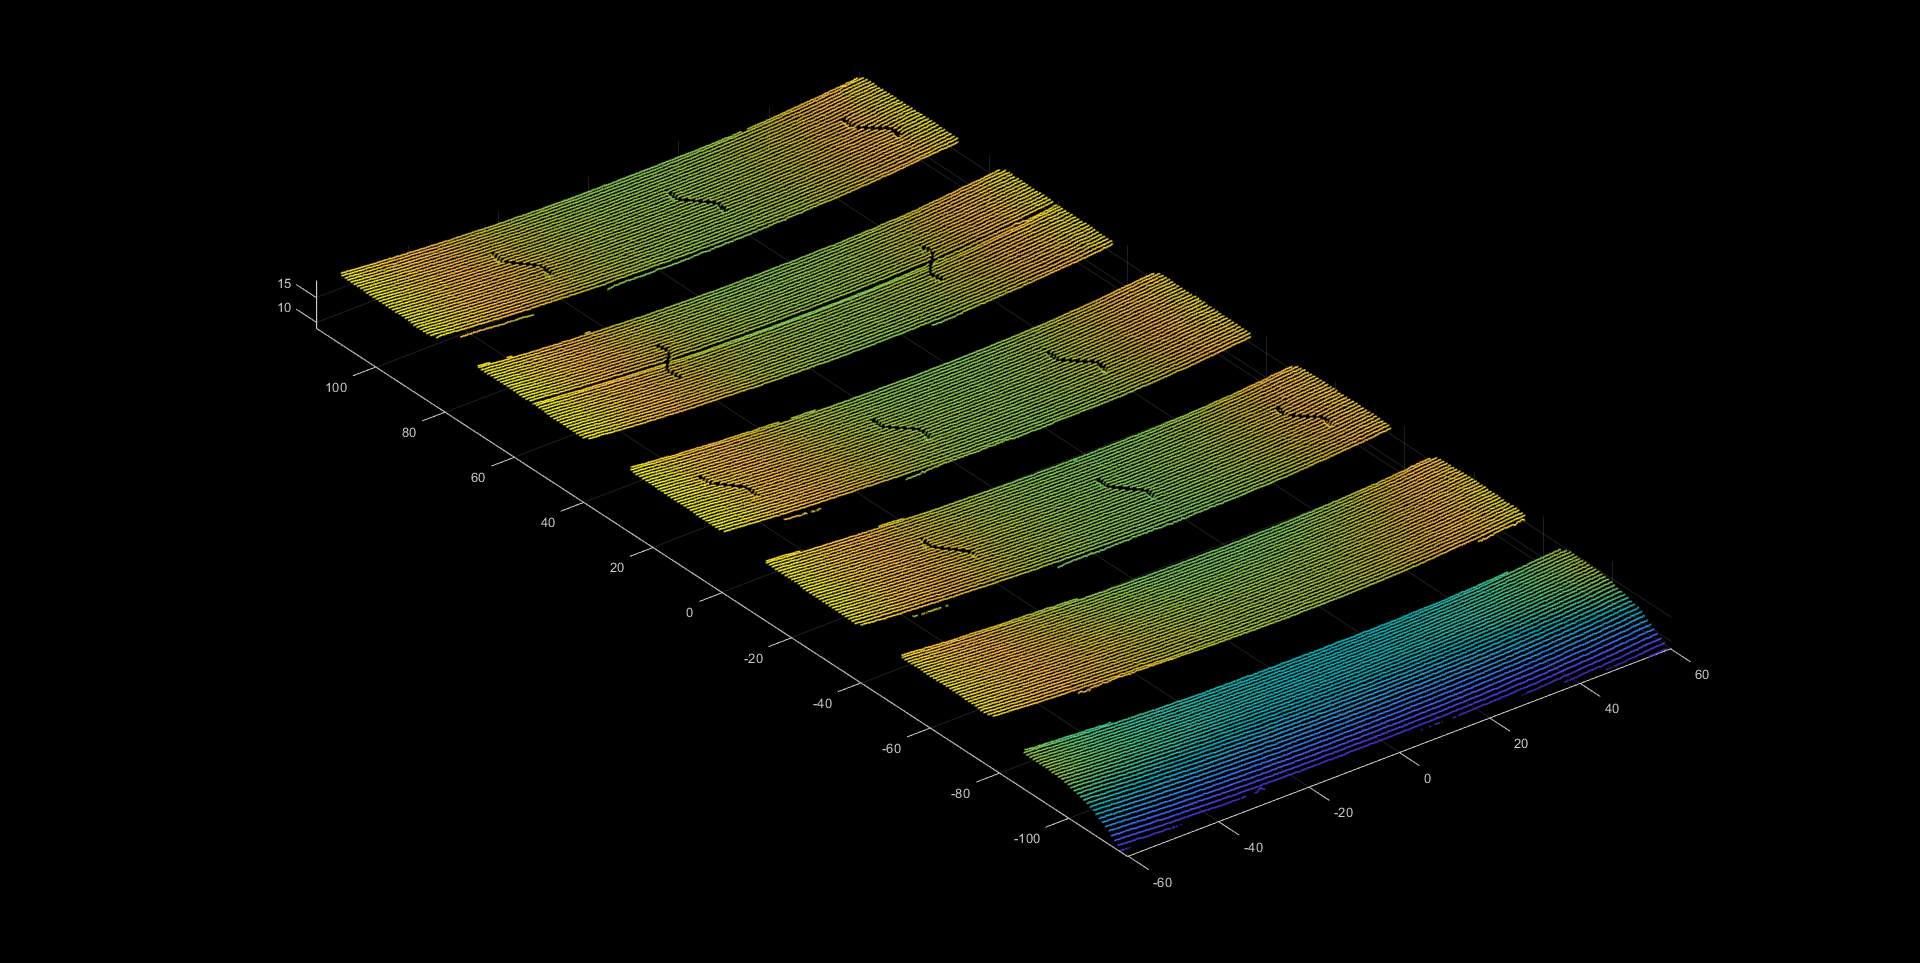
\includegraphics[width=0.45\columnwidth]{./pictures/batt_1b_analisi_2_3.png}
	\caption{Point cloud del battistrada di tipo \textit{1B} dopo aver applicato la segmentazione planare.}\label{fig:batt_1b_analisi_3}
\end{figure}

\begin{figure}[H]
	\centering
	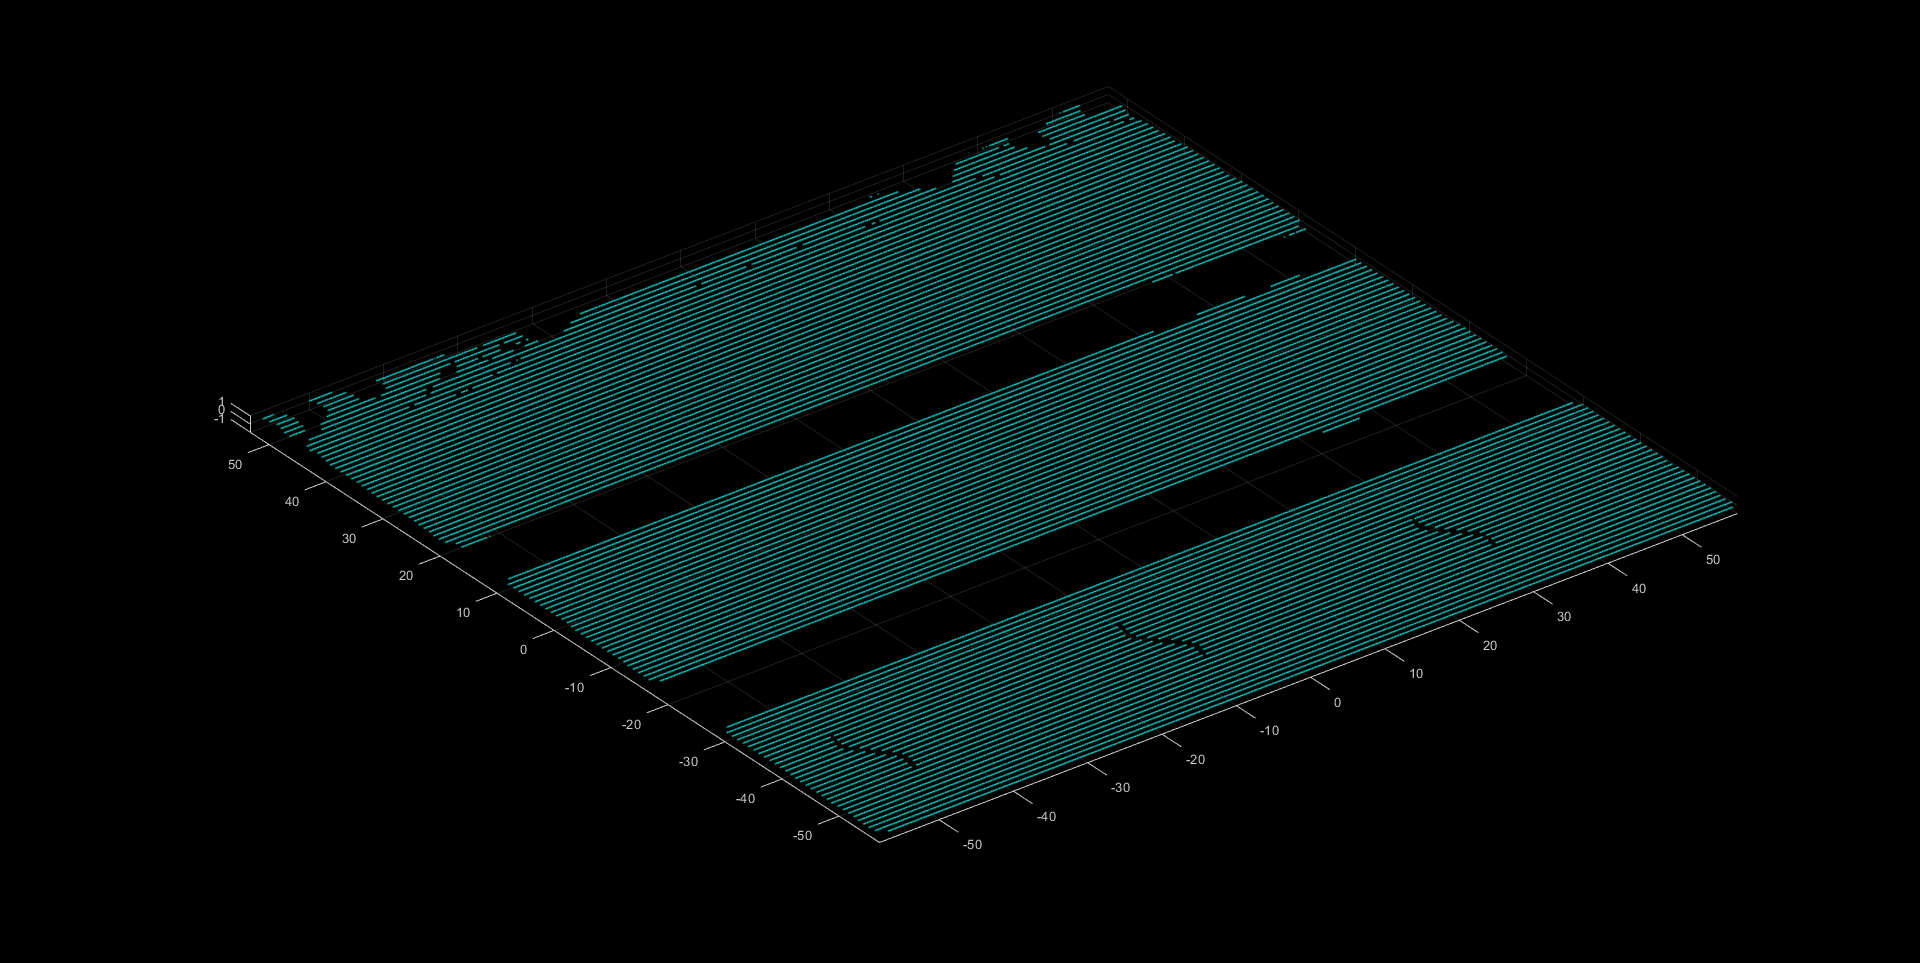
\includegraphics[width=0.45\columnwidth]{./pictures/batt_1b_analisi_1_4.png}
	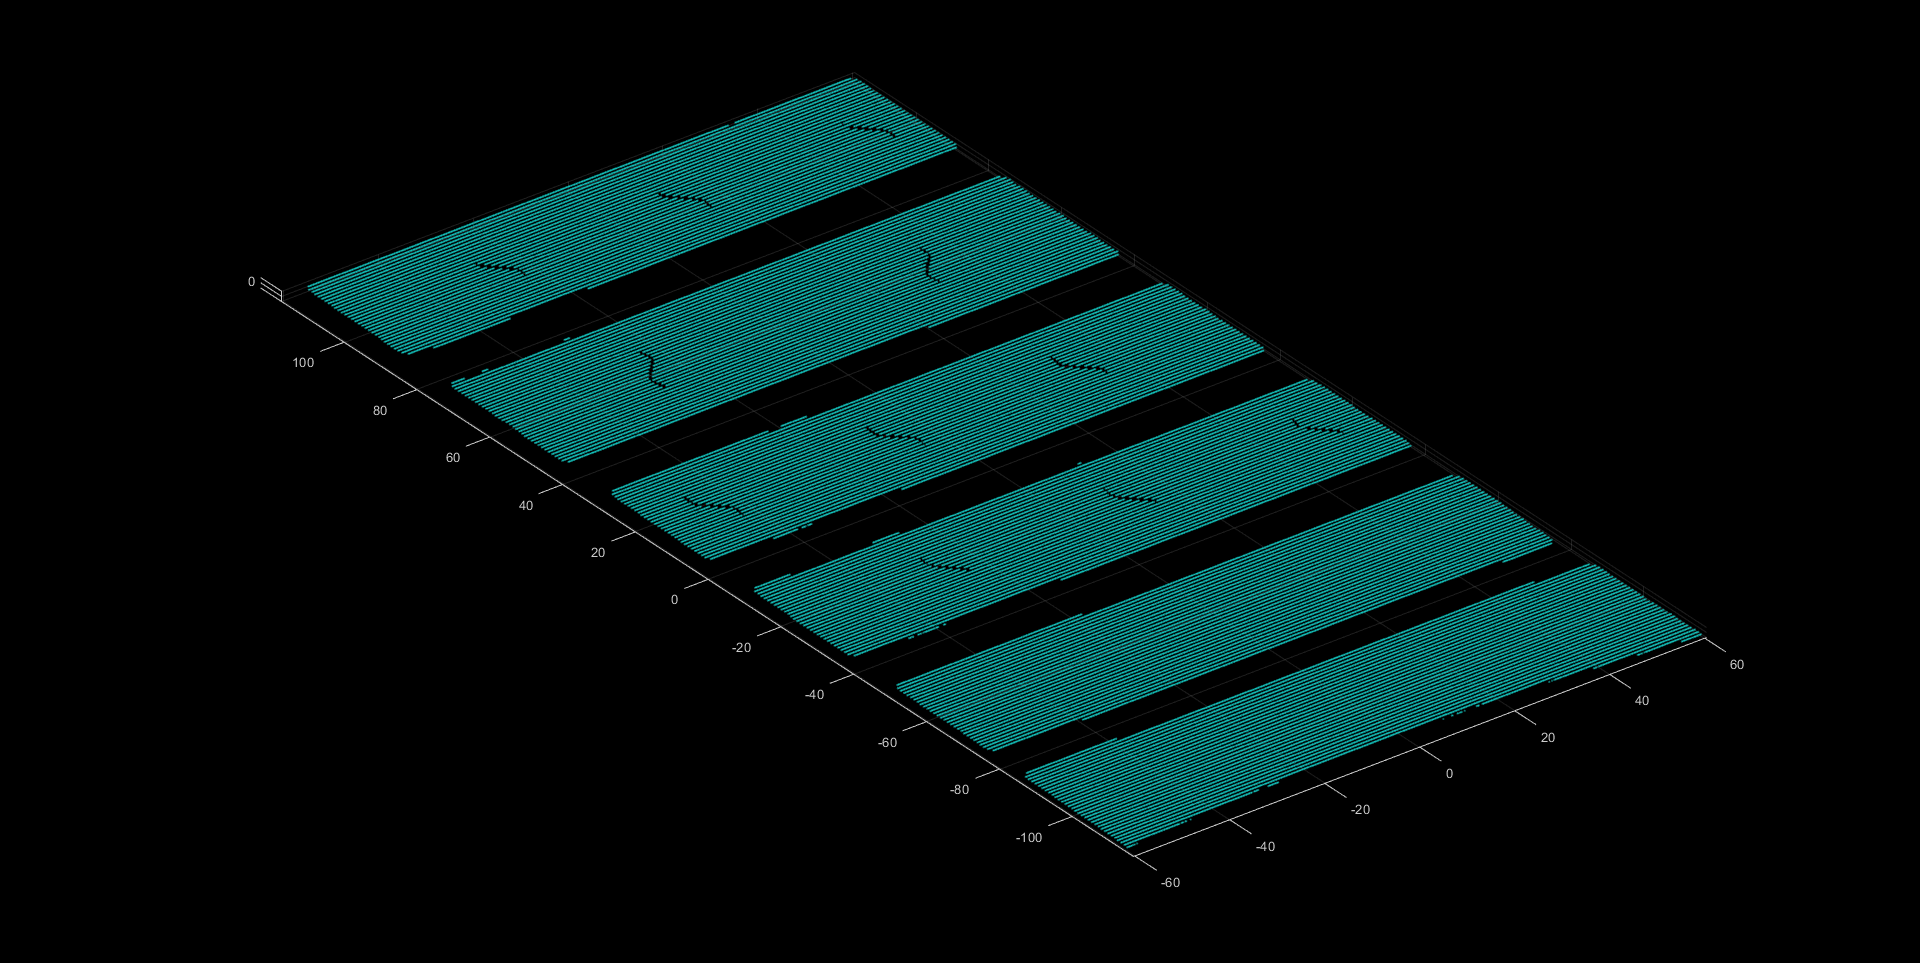
\includegraphics[width=0.45\columnwidth]{./pictures/batt_1b_analisi_2_4.png}
	\caption{Point cloud del battistrada di tipo \textit{1B} dopo aver applicato l'operazione di proiezione.}\label{fig:batt_1b_analisi_4}
\end{figure}

\begin{figure}[H]
	\centering
	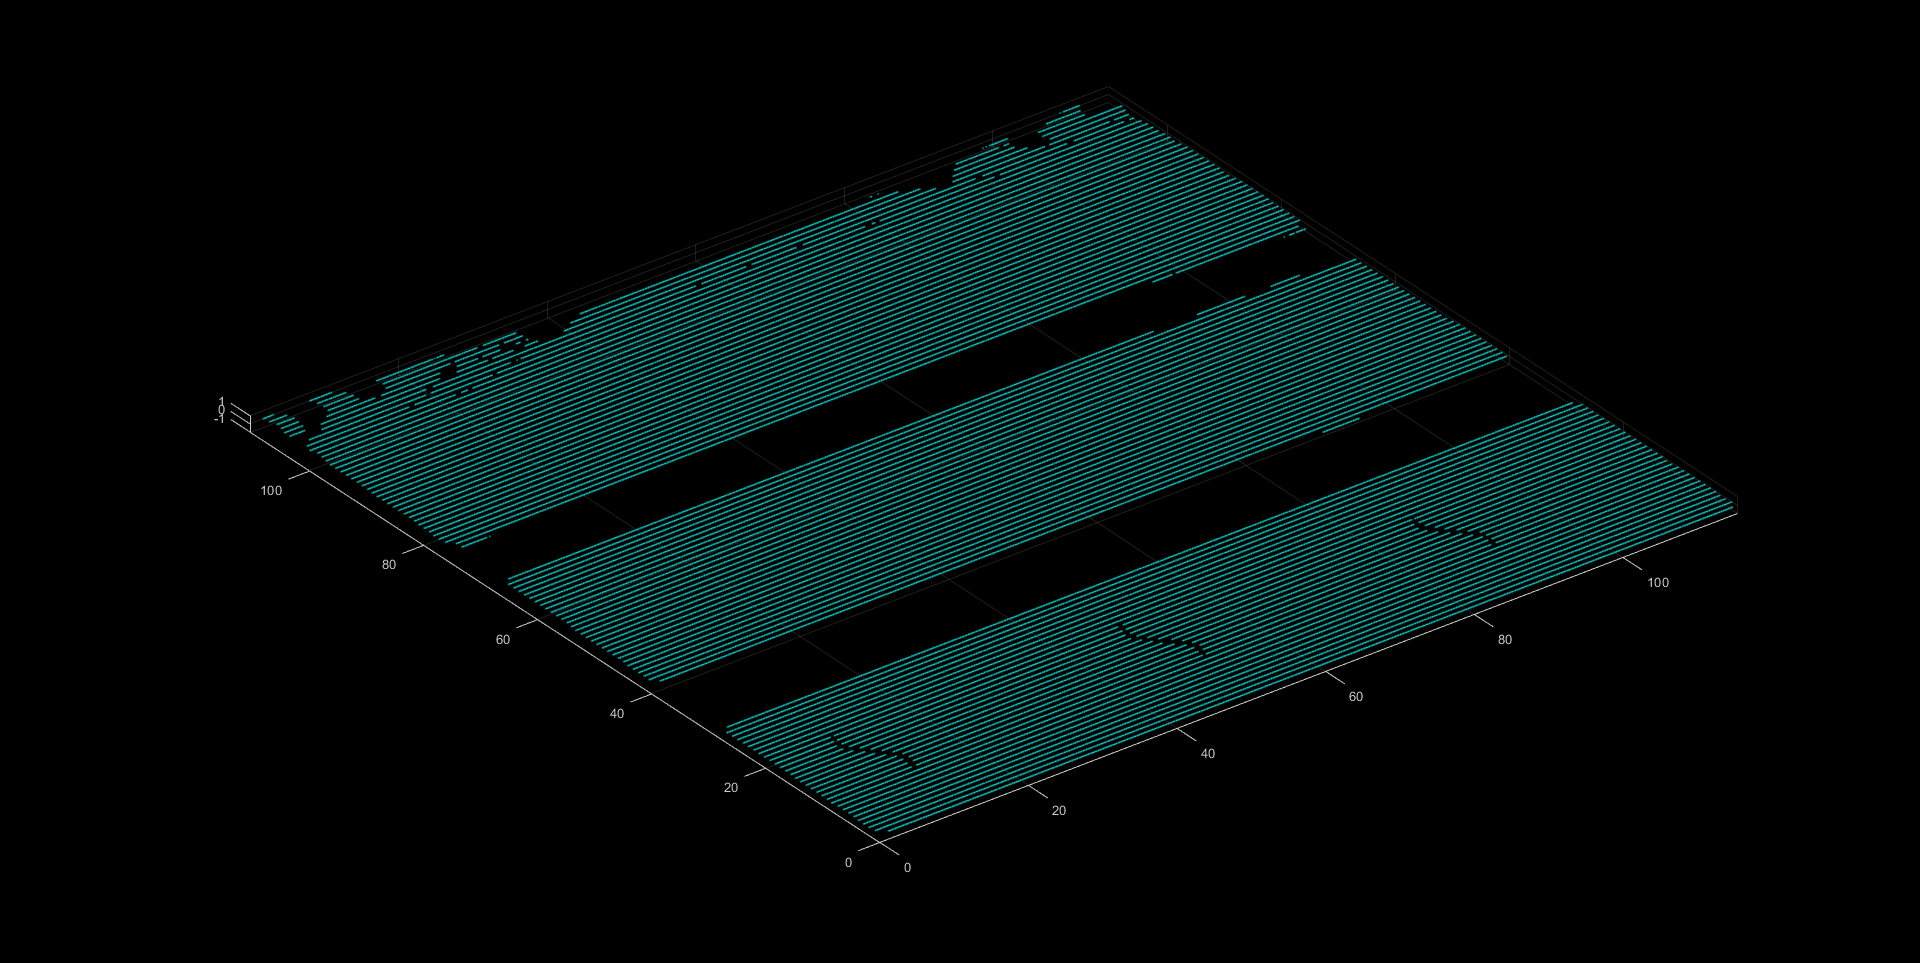
\includegraphics[width=0.45\columnwidth]{./pictures/batt_1b_analisi_1_5.png}
	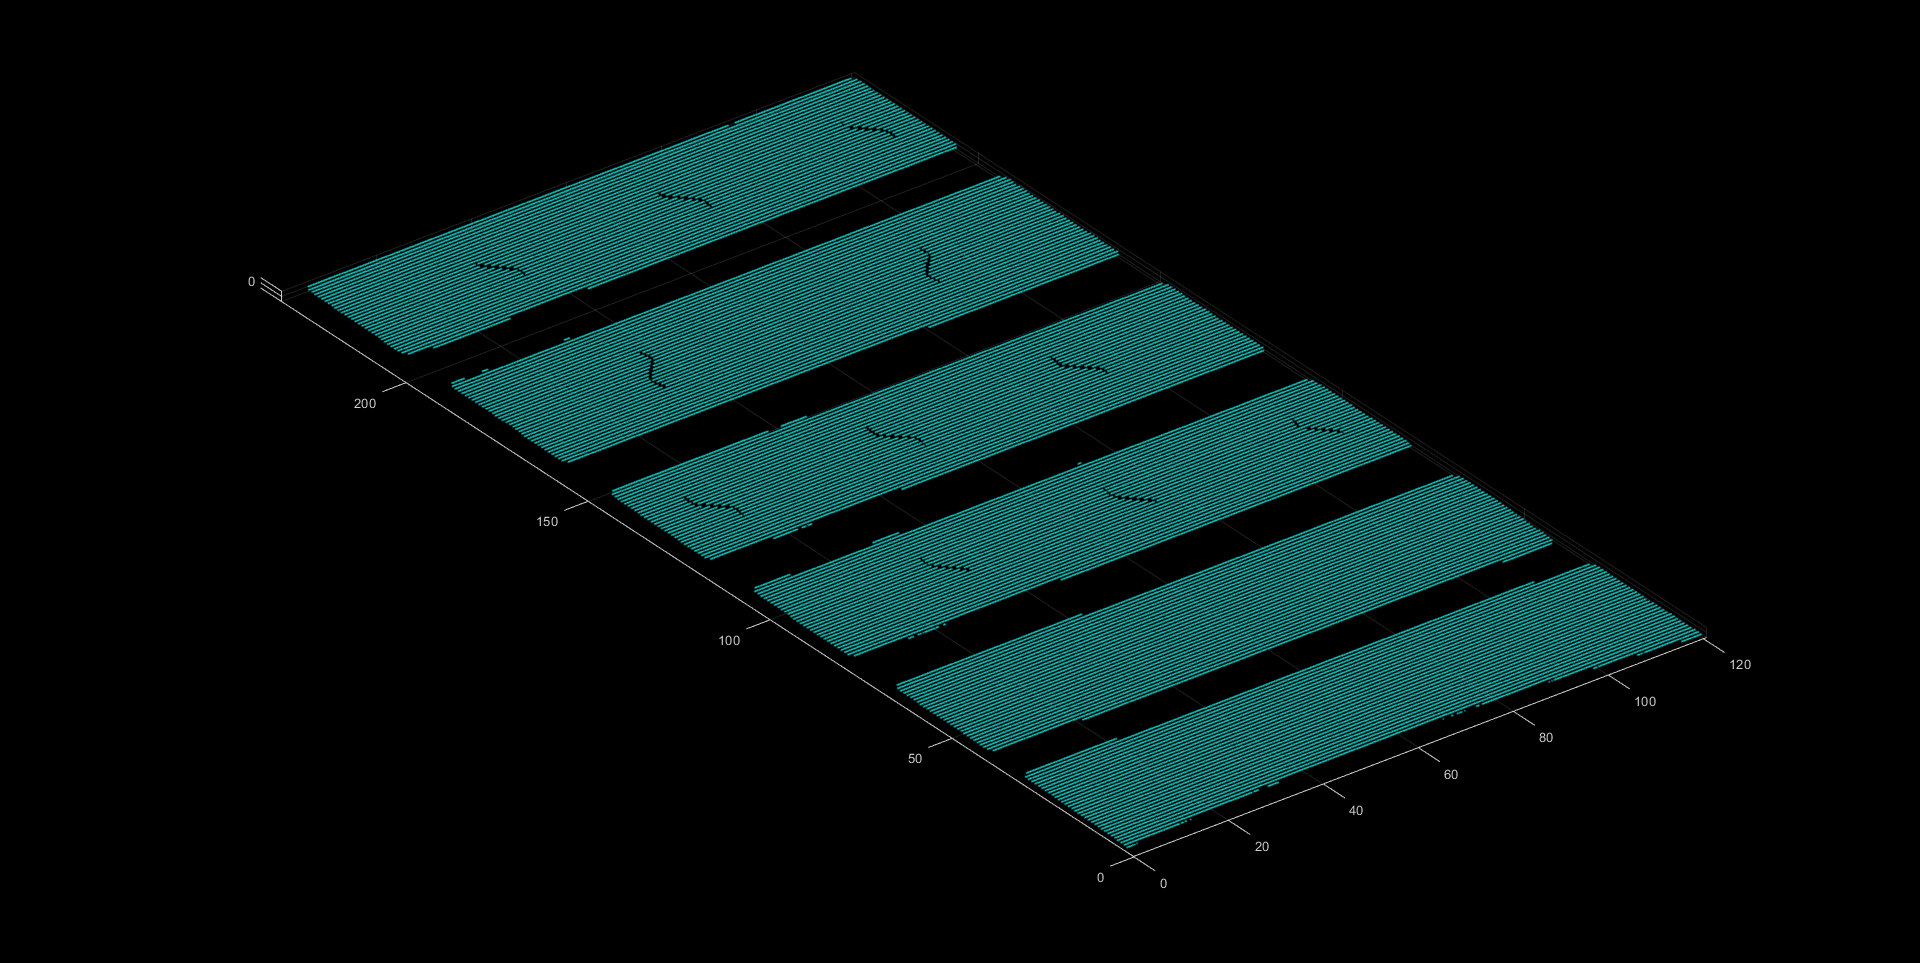
\includegraphics[width=0.45\columnwidth]{./pictures/batt_1b_analisi_2_5.png}
	\caption{Point cloud del battistrada di tipo \textit{1B} dopo aver applicato l'operazione di traslazione.}\label{fig:batt_1b_analisi_5}
\end{figure}

\begin{figure}[H]
	\centering
	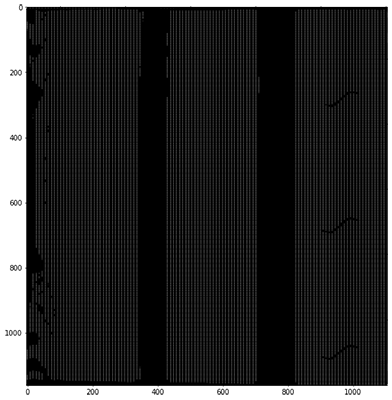
\includegraphics[height=0.32\columnwidth]{./pictures/batt_1b_analisi_1_6.png}
	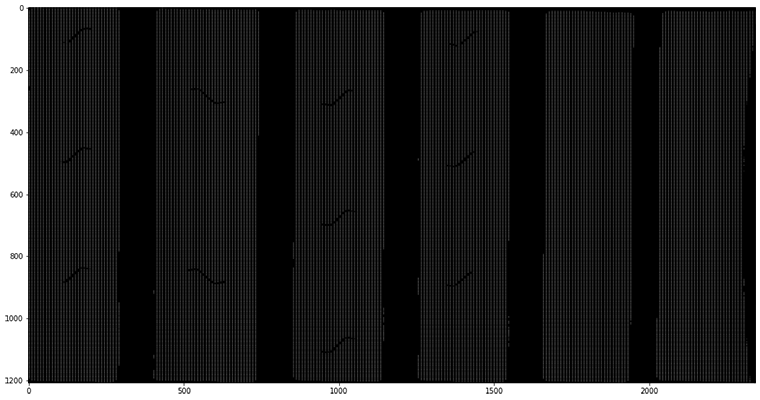
\includegraphics[height=0.32\columnwidth]{./pictures/batt_1b_analisi_2_6.png}
	\caption{Immagine planare del battistrada di tipo \textit{1B}.}\label{fig:batt_1b_analisi_6}
\end{figure}

\begin{figure}[H]
	\centering
	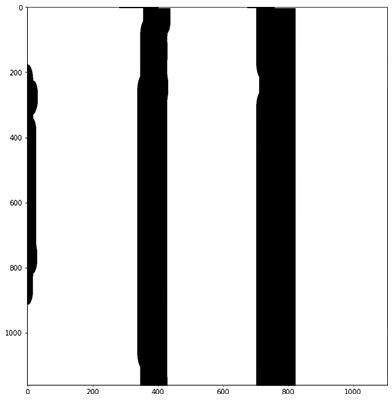
\includegraphics[height=0.32\columnwidth]{./pictures/batt_1b_analisi_1_7.png}
	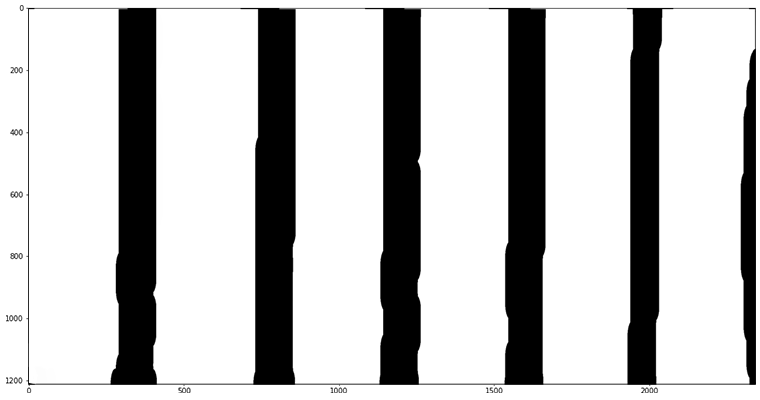
\includegraphics[height=0.32\columnwidth]{./pictures/batt_1b_analisi_2_7.png}
	\caption{Immagine del battistrada di tipo \textit{1B} dopo aver applicato la trasformazione morfologica (Closing).}\label{fig:batt_1b_analisi_7}
\end{figure}

\begin{figure}[H]
	\centering
	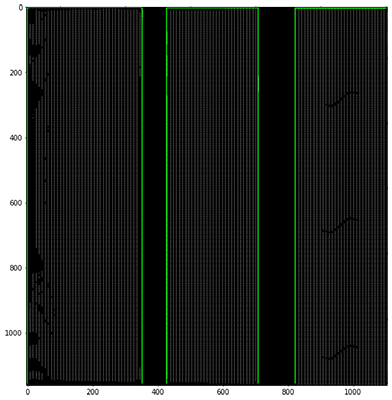
\includegraphics[height=0.32\columnwidth]{./pictures/batt_1b_analisi_1_8.png}
	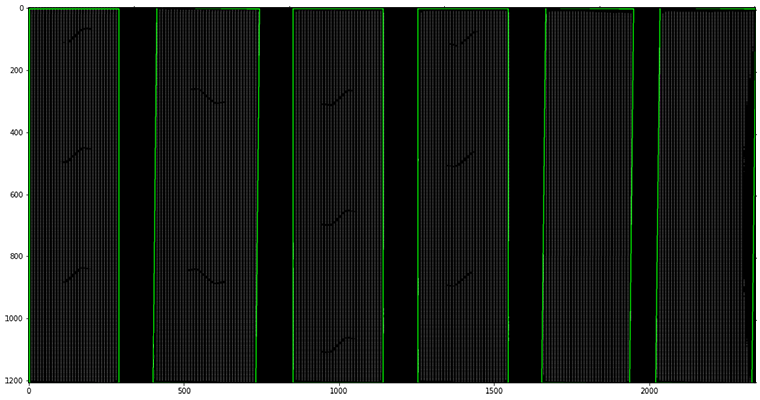
\includegraphics[height=0.32\columnwidth]{./pictures/batt_1b_analisi_2_8.png}
	\caption{Immagine del battistrada di tipo \textit{1B} con le bounding box dei MacroBlob evidenziate.}\label{fig:batt_1b_analisi_8}
\end{figure}


\subsection{Battistrada di tipo 2}
L'analisi di questo tipo di battistrada ha l'obiettivo di estrarre le seguenti features:
\begin{itemize}
	\item Misura della profondità delle scalanature presenti.
	\item Valore minimo, massimo e medio delle profondità.
\end{itemize}

\noindent Come per i battistrada precedenti, in seguito alla scansione dell'oggetto, anche in questo caso viene generata una \textit{point cloud} (figura \ref{fig:batt_2_analisi_1}).\\

\begin{figure}[H]
	\centering
	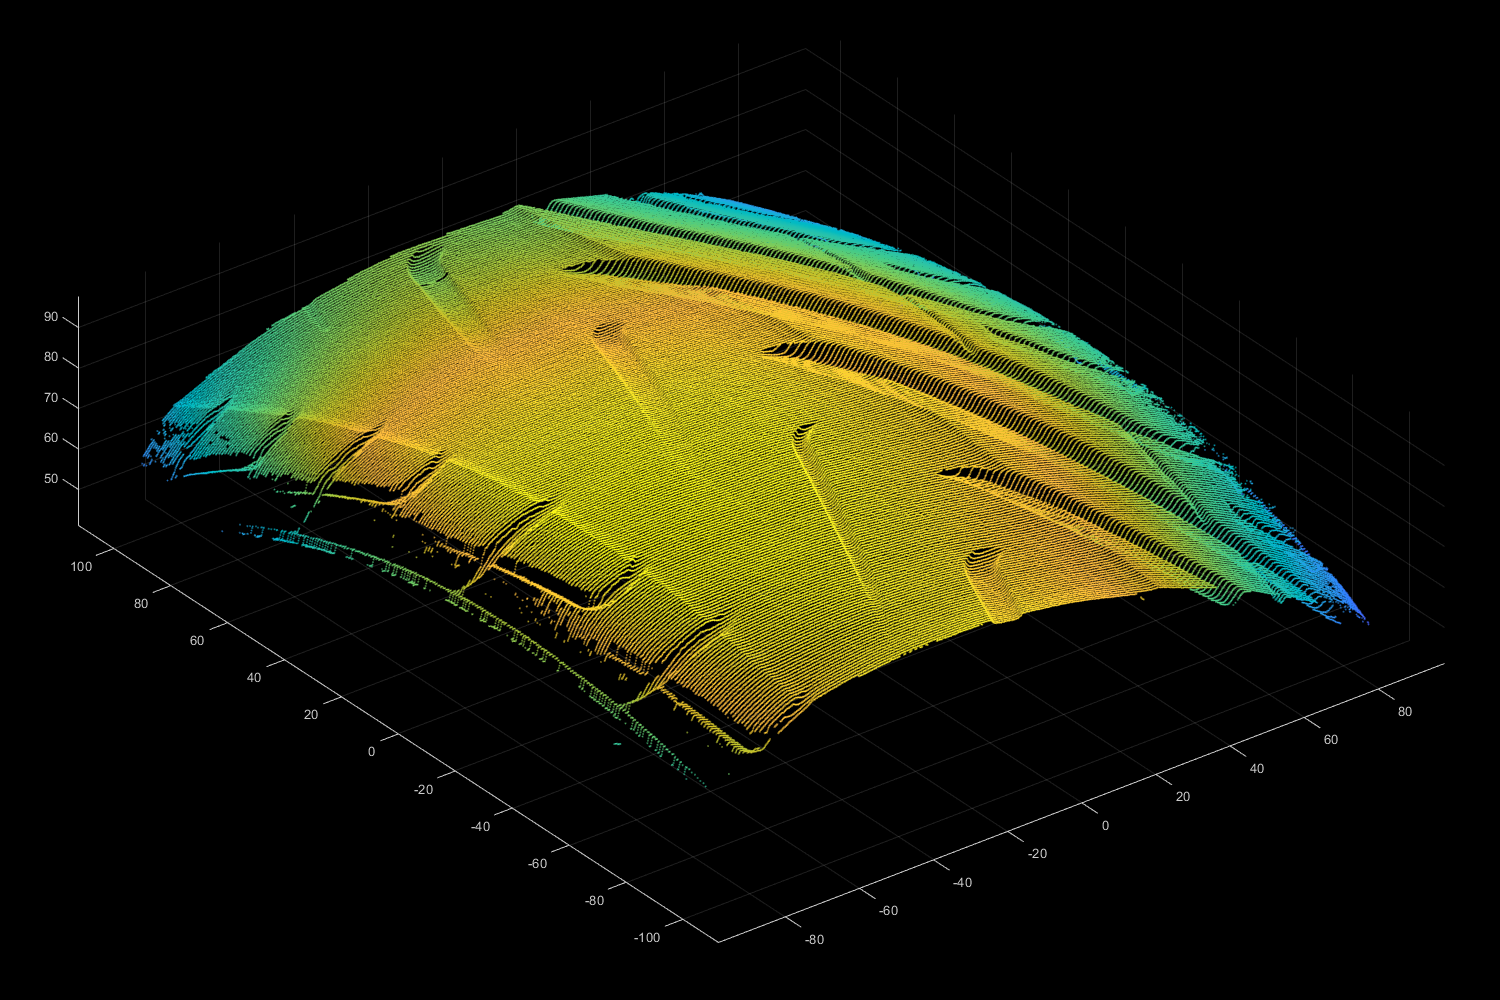
\includegraphics[width=0.45\columnwidth]{./pictures/batt_2_analisi_1.png}
	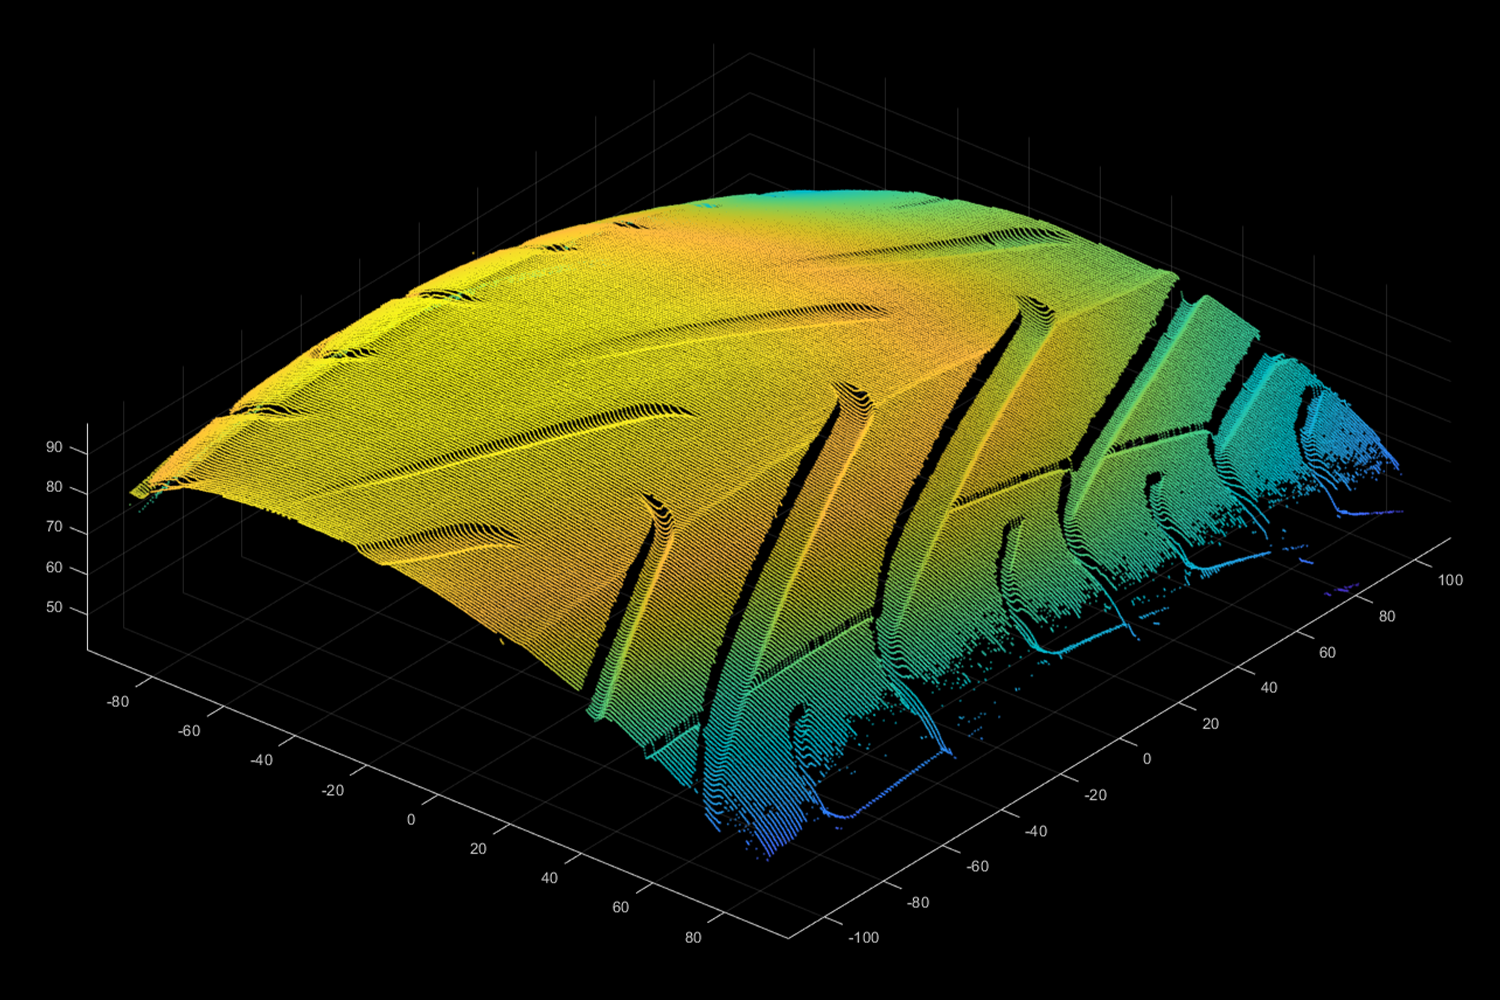
\includegraphics[width=0.45\columnwidth]{./pictures/batt_2_analisi_2.png}
	\caption{Point cloud non elaborata del battistrada di tipo \textit{2}.}\label{fig:batt_2_analisi_1}
\end{figure}

\noindent Per determinare la profondità del battistrada del pneumatico in modo accurato e automatico, è stato sviluppato un metodo di misurazione che prima identifica la posizione delle scanalature e poi calcola, in successione, le profondità di ciascun solco.\\
\newline
L'approccio che si è seguito è quello di scansionare l'intera \textit{point cloud} lungo l'asse \textit{y}, linea per linea, in modo da avere \textit{n} funzioni polinomiali che concatenate ricreino l'intera \textit{point cloud}.\\

\begin{figure}[H]
	\centering
	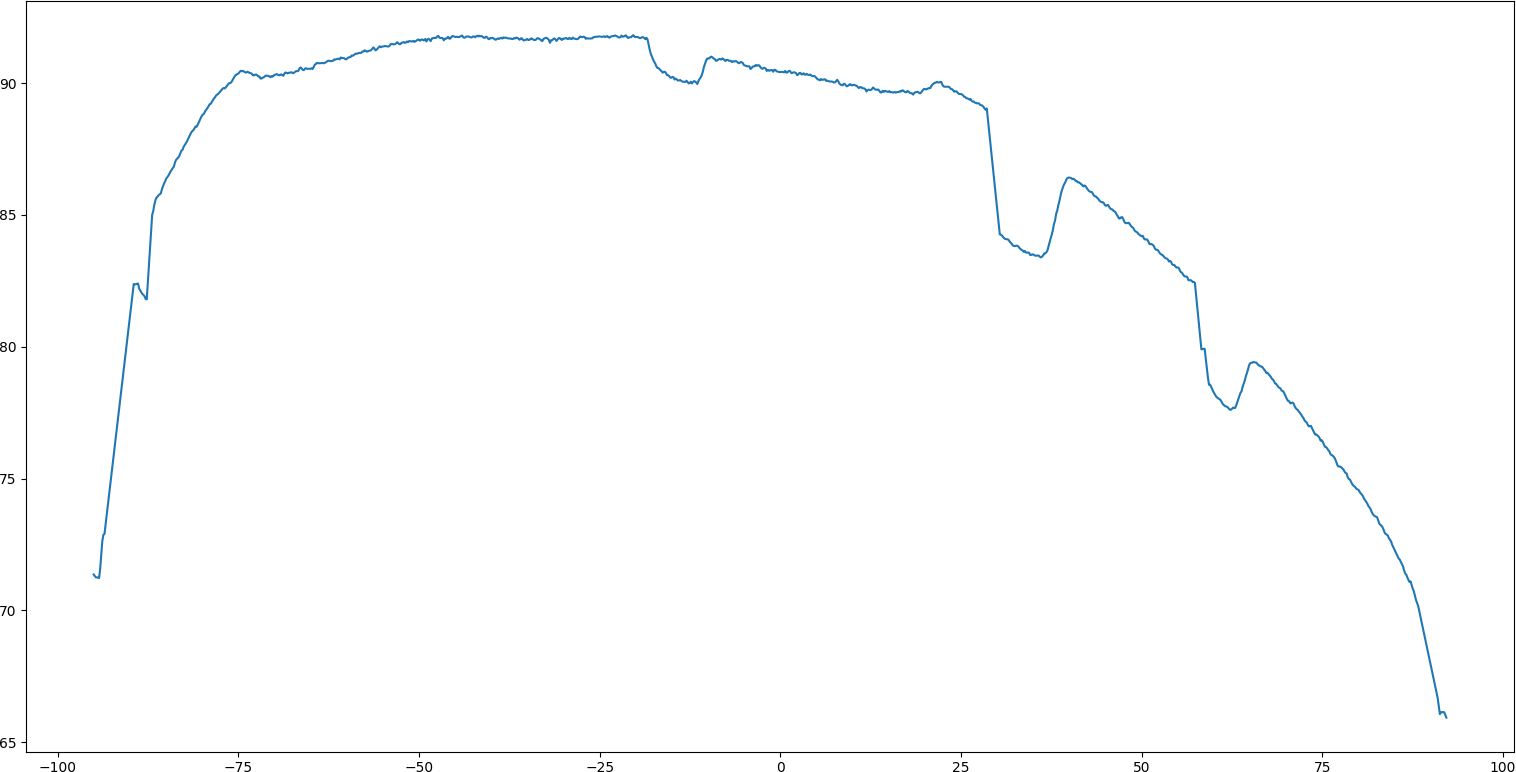
\includegraphics[width=0.9\columnwidth]{./pictures/batt_2_analisi_3.png}
	\caption{Funzione originale.}\label{fig:batt_2_analisi_3}
\end{figure}

\begin{figure}[H]
	\centering
	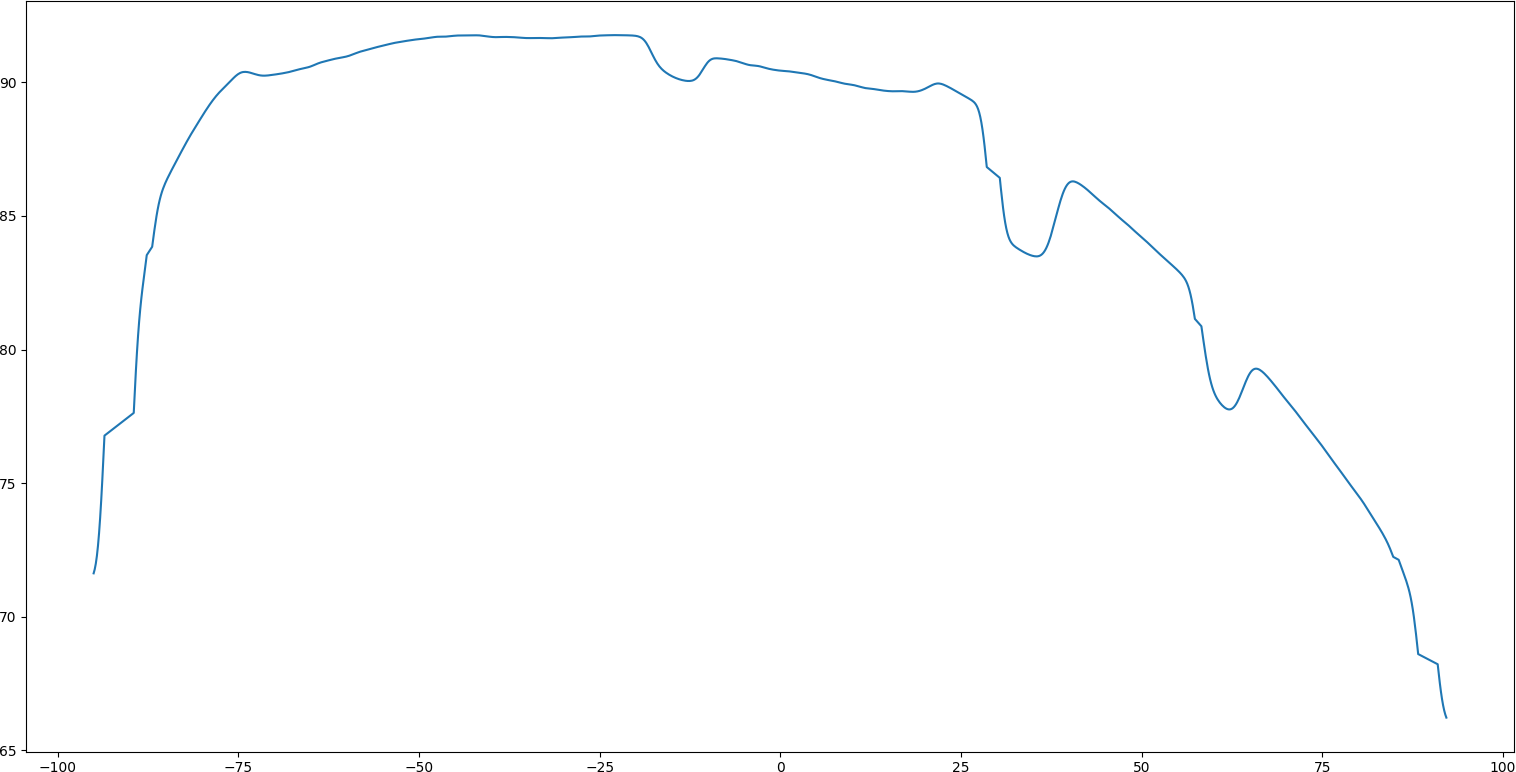
\includegraphics[width=0.9\columnwidth]{./pictures/batt_2_analisi_4.png}
	\caption{Funzione smussata.}\label{fig:batt_2_analisi_4}
\end{figure}

\noindent Per spiegare l'algoritmo prendiamo come esempio una delle \textit{n} funzioni processate. Come si può notare dalla figura \ref{fig:batt_2_analisi_3}, oltre alle scanalature di grandi dimensioni presenti sulla superficie del pneumatico, sono presenti scanalature molto piccole (dovute alla rumorosità) che potrebbero trarre in inganno l'algoritmo di ricerca.\\
\newline
Le scanalature più piccole possono essere rimosse dalla curva del profilo applicando un filtro gaussiano, in modo da rendere la funzione  più smussata (figura \ref{fig:batt_2_analisi_4}). Dopo una serie di prove, come parametri del filtro, sono stati scelti una finestra \textit{$K$ = 51} (dimensione del kernel) e un \textit{$\alpha$ = 5} che specifica il numero di deviazioni standard $\sigma$ desiderate nel kernel.\\
\newline
Ora che la funzione originale è stata smussata, per trovare la posizione e la misura della profondità delle scanalature, ci viene in soccorso lo studio della derivata e dei punti di flesso.\\
\newline
Infatti, tra due punti di massimo della funzione smussata (figura \ref{fig:batt_2_analisi_5}), si trova obbligatoriamente una scanalatura del battistrada, e la profondità di ciascuna scanalatura è data dalla massima distanza che va dal fondo concavo, alla linea che congiunge i due punti di massimo.\\
\newline
Una volta trovati i punti critici nella funzione smussata, sono state salvate le rispettive coordinate \textit{x} di ogni punto e riportate nella funzione originale (figura \ref{fig:batt_2_analisi_6} e figura \ref{fig:batt_2_analisi_7}).\\

\begin{figure}[H]
	\centering
	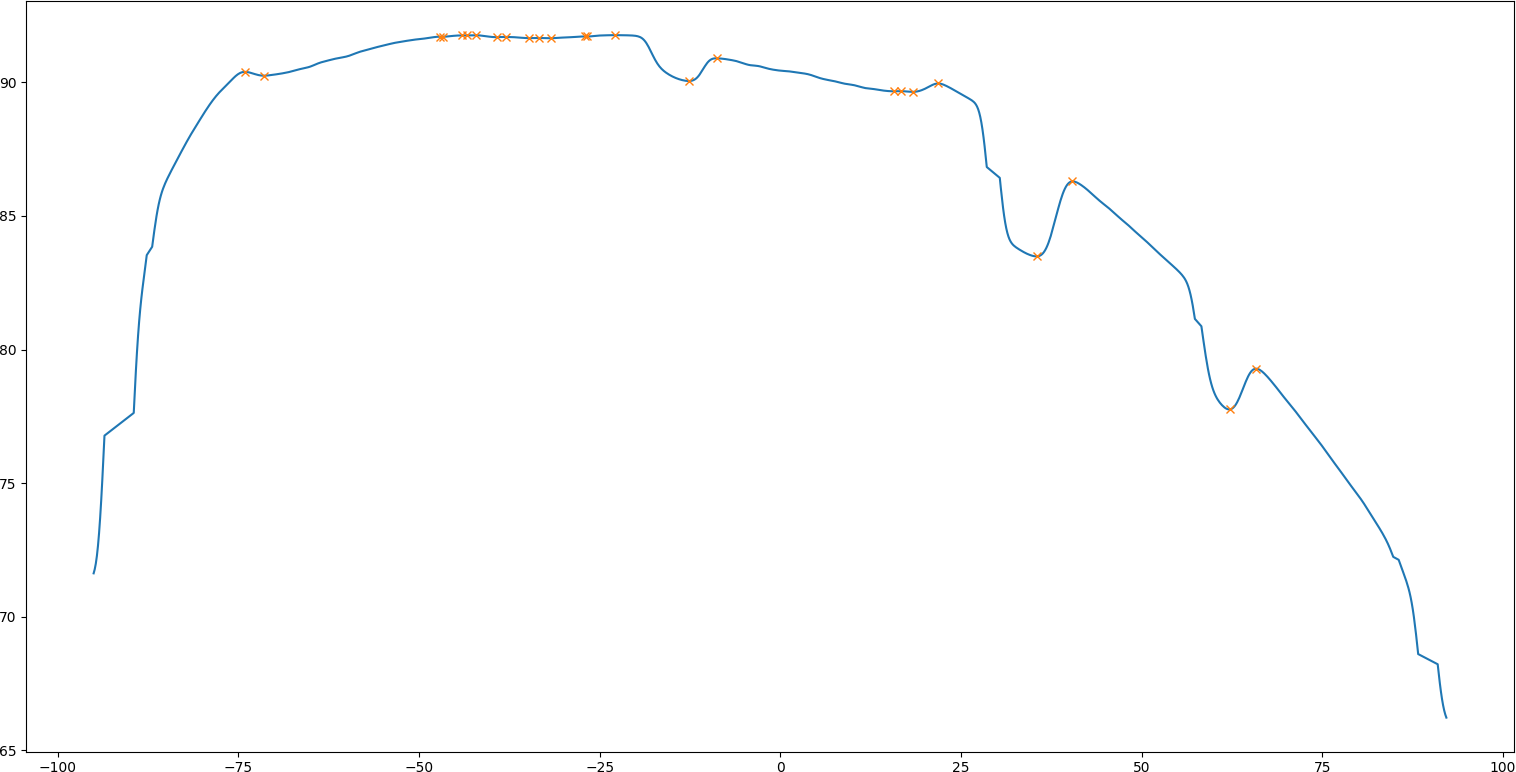
\includegraphics[width=0.9\columnwidth]{./pictures/batt_2_analisi_5.png}
	\caption{Massimi e minimi della funzione smussata.}\label{fig:batt_2_analisi_5}
\end{figure}

\begin{figure}[H]
	\centering
	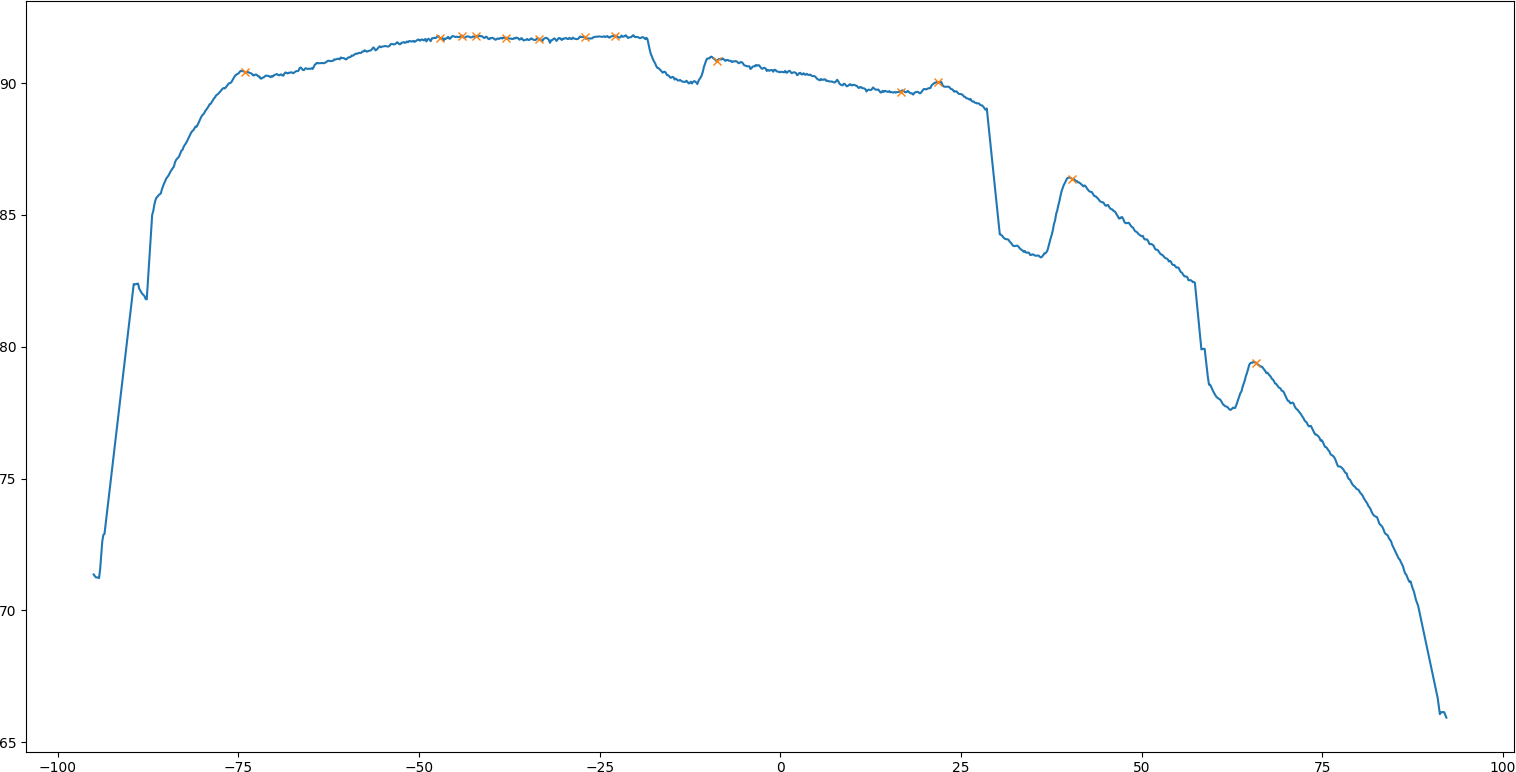
\includegraphics[width=0.9\columnwidth]{./pictures/batt_2_analisi_6.png}
	\caption{Massimi (da destra) della funzione originale.}\label{fig:batt_2_analisi_6}
\end{figure}

\begin{figure}[H]
	\centering
	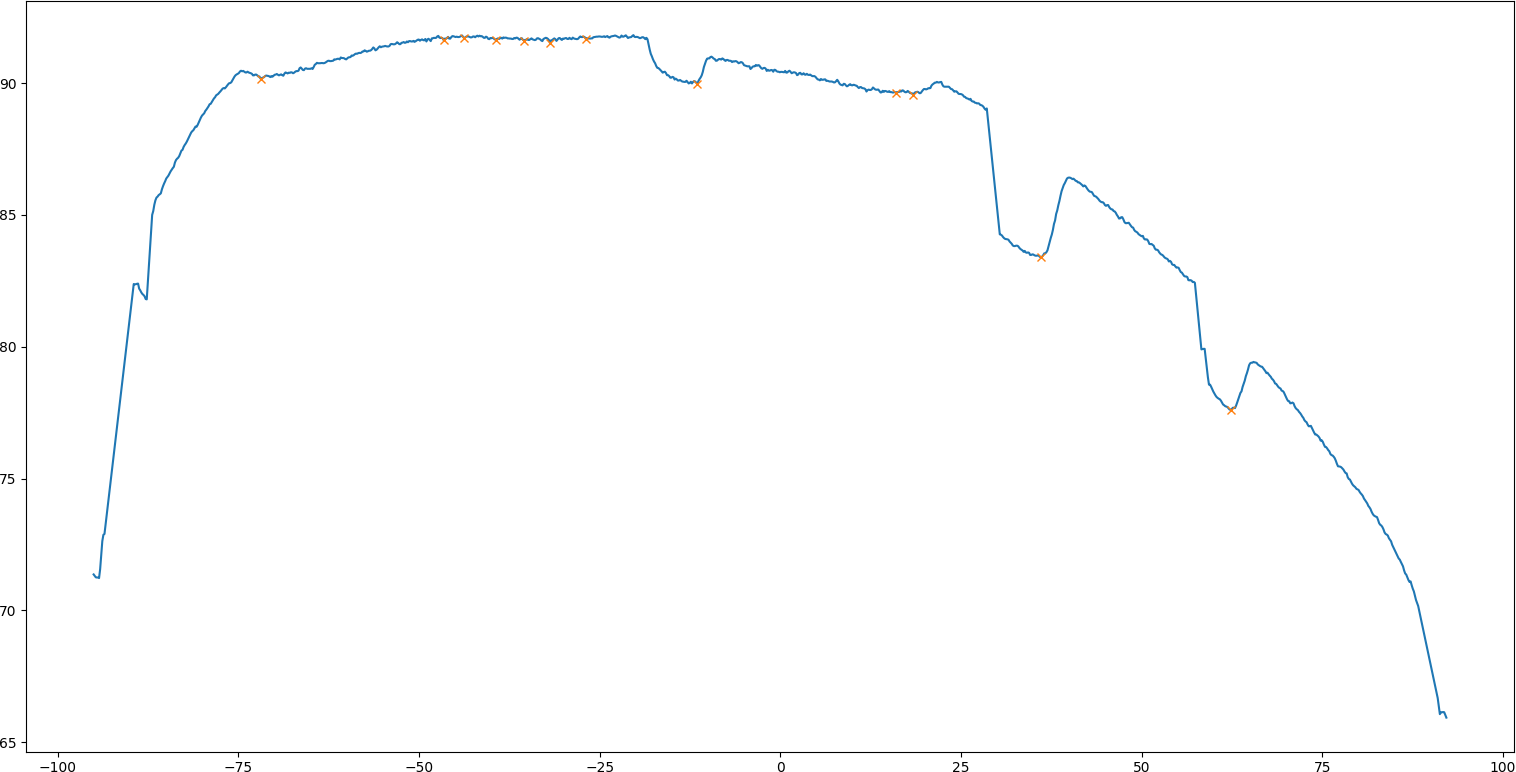
\includegraphics[width=0.9\columnwidth]{./pictures/batt_2_analisi_7.png}
	\caption{Minimi della funzione originale.}\label{fig:batt_2_analisi_7}
\end{figure}

\noindent Seguendo il percorso del profilo del battistrada, a partire dall'estrema destra, ciò che abbiamo trovato fino ad ora sono: il punto dove inizia la scanalatura, il punto più profondo di essa e il punto dove inizia l'eventuale scanalatura successiva.\\
\newline
Quindi, per migliorare la precisione della posizione delle scanalature, dobbiamo trovare la posizione del punto di chiusura di ogni scanalatura.
\newpage
\noindent Per trovare questi punti, che chiameremo impropriamente punti di massimo da sinistra, si è seguito il seguente algoritmo:

\begin{itemize}
	\item Isolare la parte di funzione che si trova tra un minimo e il massimo successivo;
	\item Ruotarla, facendo in modo che la retta passante tra il minimo e il massimo sia parallela all'asse delle \textit{x};
	\item Individuare il punto di massimo della porzione di funzione ruotata, che in definitiva sarà il nostro massimo da sinistra;
\end{itemize}

\noindent Così facendo si trova un buon punto di massimo approssimato, dato che la rotazione non intacca la posizione dei punti.\\
\newline
Nella figura \ref{fig:batt_2_analisi_8} è illustrato un esempio di questo calcolo, con evidenziate di verde, sia la funzione smussata sia quella ruotata, da cui si è individuato il nostro punto di massimo.\\
\newline
Una volta ripetuto l'algoritmo per ogni tratto della funzione smussata, la posizione di ogni punto di massimo trovata, è stata riportata nella funzione originale (figura \ref{fig:batt_2_analisi_9}).\\

\begin{figure}[H]
	\centering
	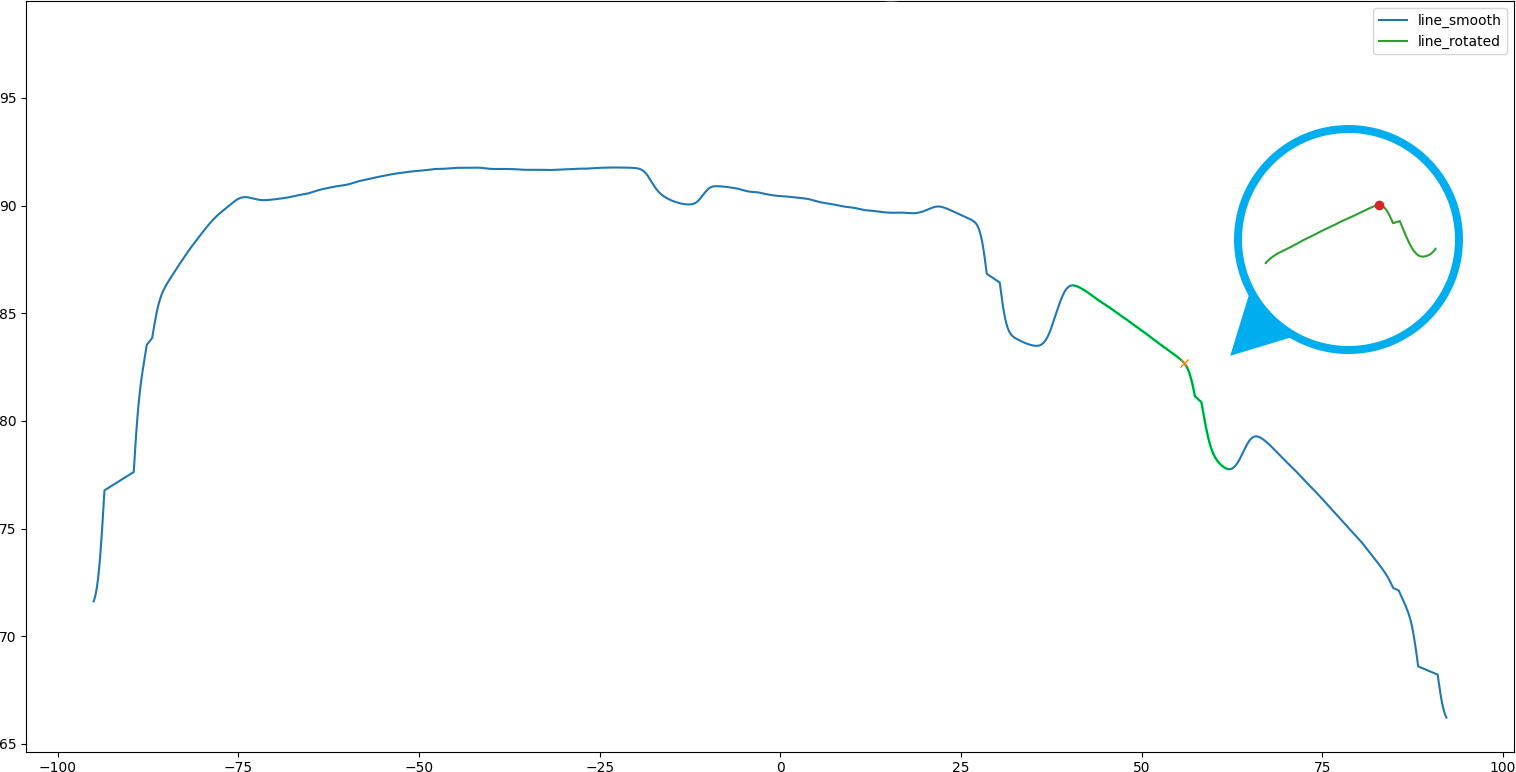
\includegraphics[width=0.9\columnwidth]{./pictures/batt_2_analisi_8.png}
	\caption{Esempio del calcolo di uno dei massimi (da sinistra) della funzione smussata.}\label{fig:batt_2_analisi_8}
\end{figure}

\begin{figure}[H]
	\centering
	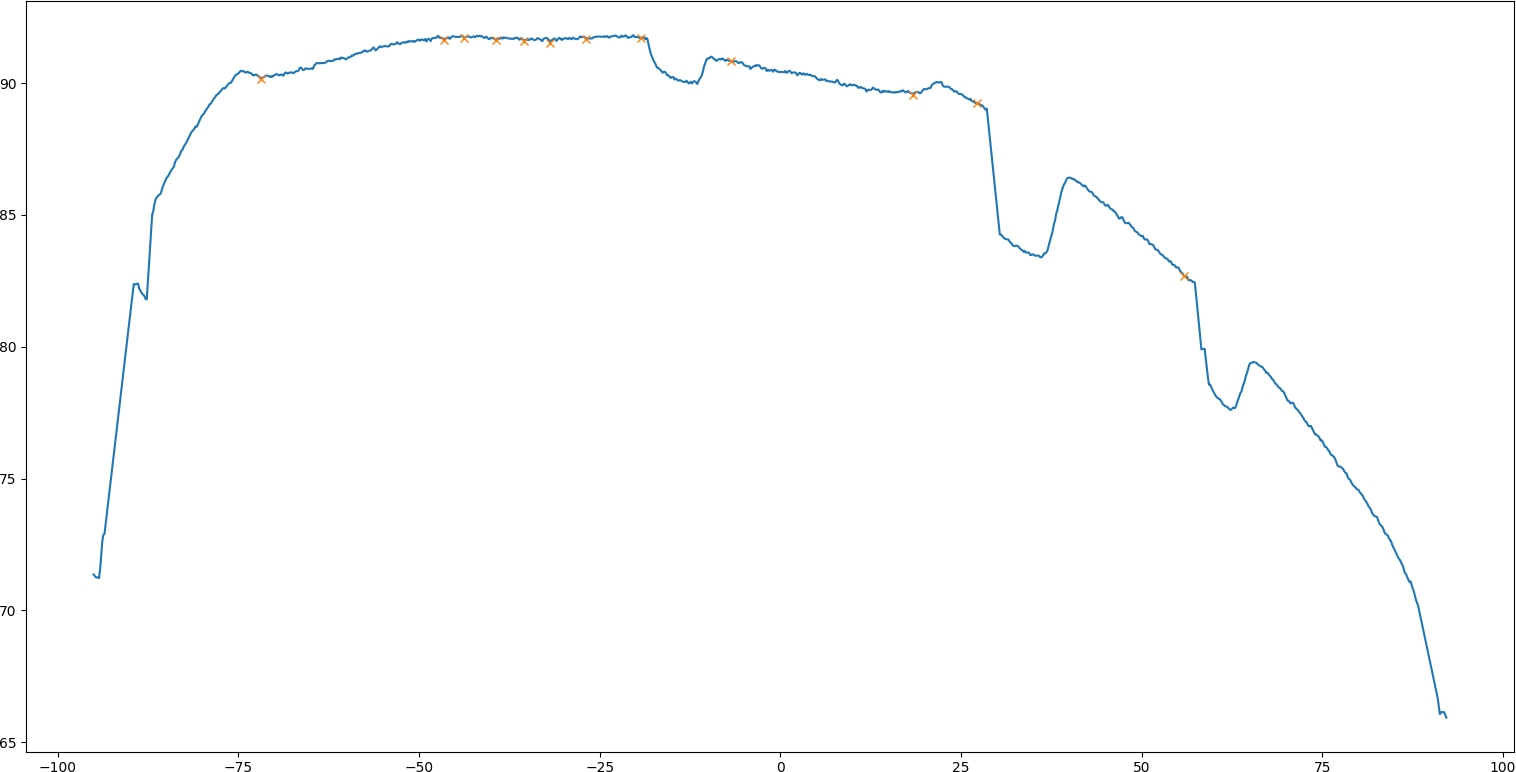
\includegraphics[width=0.9\columnwidth]{./pictures/batt_2_analisi_9.png}
	\caption{Massimi (da sinistra) della funzione originale.}\label{fig:batt_2_analisi_9}
\end{figure}

\noindent Dopo aver chiarito definitivamente la posizione e il numero delle scanalature del battistrada, è possibile misurare la profondità di ciascuna scanalatura, calcolando la distanza tra la retta che congiunge un massimo da destra e un massimo da sinistra, e il punto di minimo corrispondente.\\
\newline
In fine è stato applicato un filtro, in modo tale da prendere solo le distanze che siano maggiori di 0.5 millimetri (figura \ref{fig:batt_2_analisi_10}).\\

\begin{figure}[H]
	\centering
	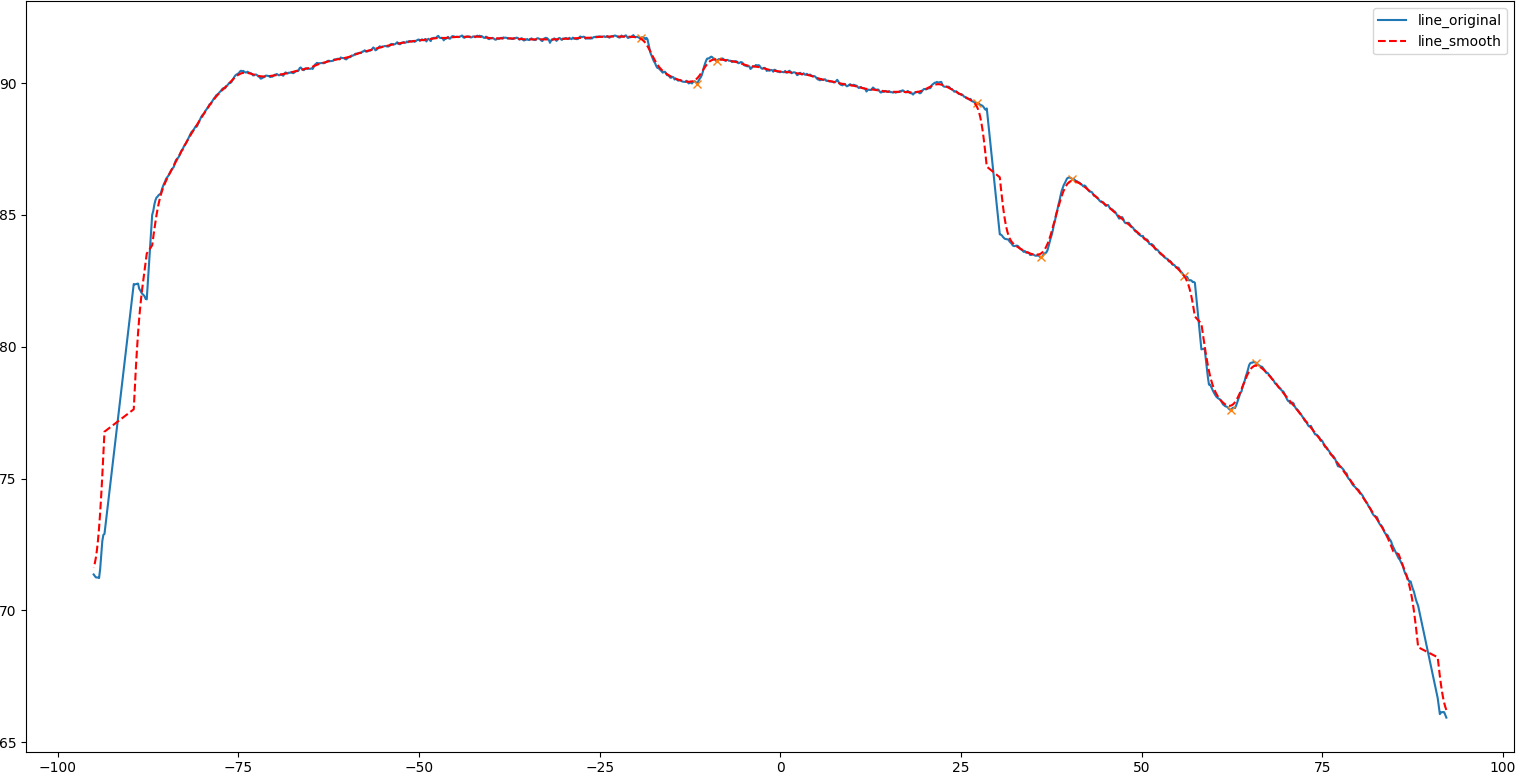
\includegraphics[width=0.9\columnwidth]{./pictures/batt_2_analisi_10.png}
	\caption{Confronto tra la funzione originale e la funzione smussata. I punti critici segnati sono il risultato di un filtro sulla distanza maggiore di 0.5 millimetri.}\label{fig:batt_2_analisi_10}
\end{figure}

\begin{figure}[H]
	\centering
	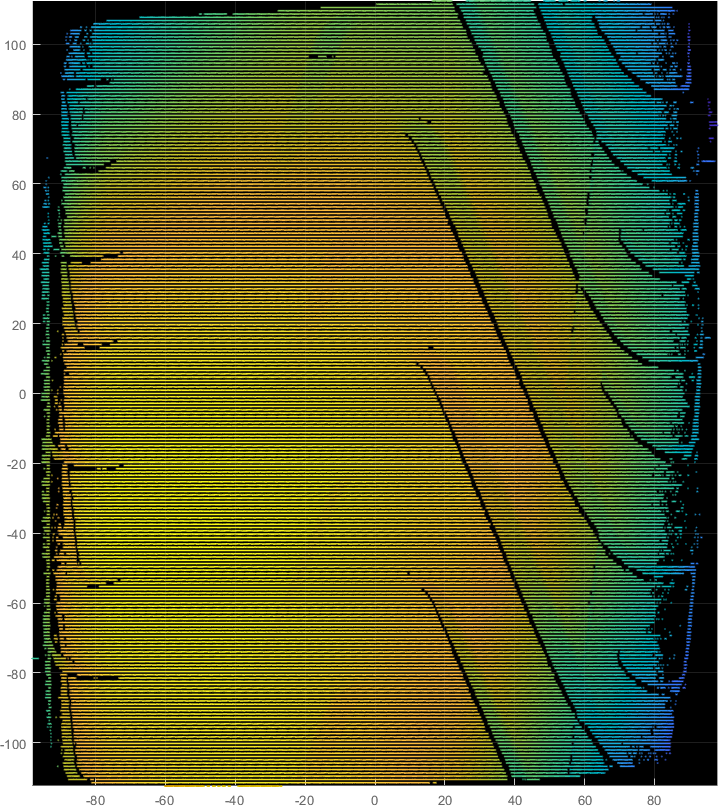
\includegraphics[width=0.5\columnwidth]{./pictures/battistrada.png}
	\caption{Point cloud del battistrada di tipo \textit{2}, con vista sul piano \textit{XY}.}\label{fig:battistrada}
\end{figure}

\begin{figure}[H]
	\centering
	\subfloat[][]{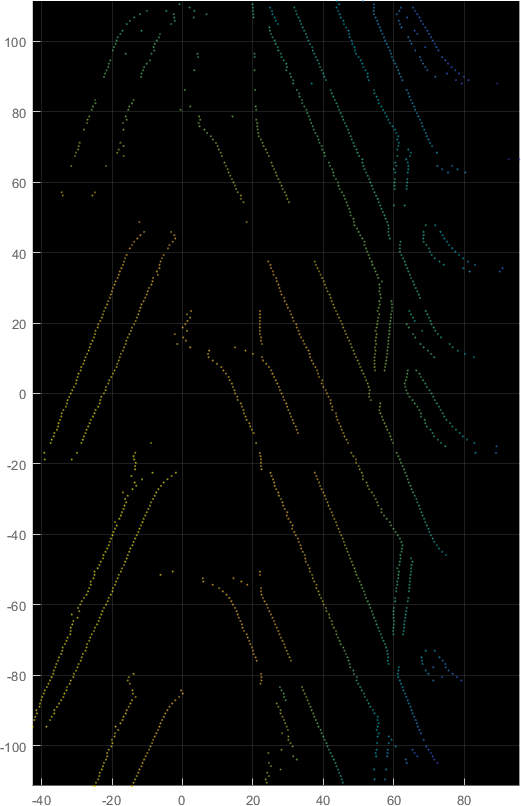
\includegraphics[height=0.6\columnwidth]{./pictures/battistrada_maxr_maxl_0.3.png}}
	\hspace{1em}
	\subfloat[][]{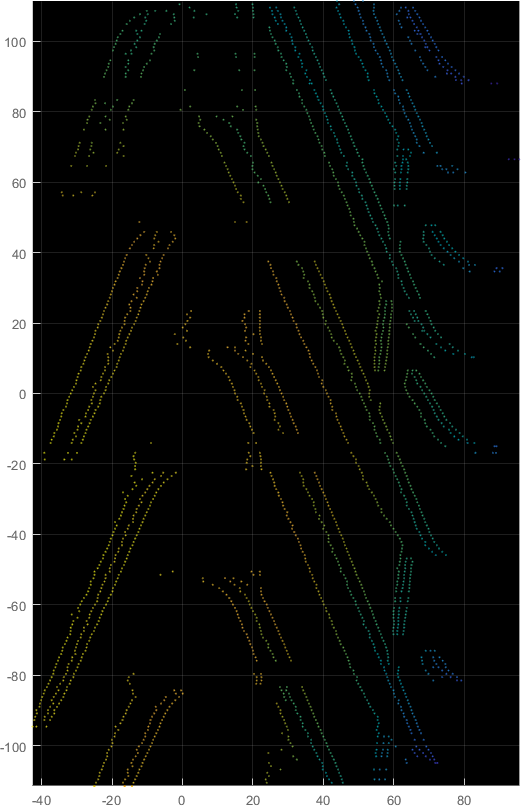
\includegraphics[height=0.6\columnwidth]{./pictures/battistrada_maxr_min_maxl_0.3.png}}
	\caption{(a) Point cloud contenente i punti di massimo da sinistra e di massimo da destra. (b) Point cloud contenente i punti di minimo, massimo da sinistra e di massimo da destra.}\label{fig:battistrada_maxr_maxl_0.3}
\end{figure}